\chapter{Calibration Hardware for Single-Phase}
\label{ch:sp-calib}

%%%%%%%%%%%%%%%%%%%%%%%%%%%%%%%%%%%%%%%%%%%%%%%%%%%%%%%
\section{Calibration Hardware Overview}
\label{sec:sp-calib-ov}

%\section{Calibration Hardware Overview}
%\label{sec:sp-calib-ov}

%\todo{Tables and figures seem to be shifted outside the sections and some not showing up. This needs Anne or other expert help...}
%\todo{SG: it seems that if you include \todo comments inside a table, it completely messes up the rest of the document. I tested this and once you remove those, figures and tables start showing up. Weird! But, now everything is in order.}
%%%%%%%%%%%%%%%%%%%%%%%%%%%%
\subsection{Introduction}
\label{sec:sp-calib-ov-intro}

\fixme{(from Nora) I must point out that the headings in this document are problematic. They go to five levels, in some places (see page 7 on the PDF) with no text until the fifth level heading. This is extremely troubling. Generally, no heading should appear without at least transitional text following it, and here we have three headings with nothing, no content, no transitions, no indications of anything. This will not do. This is especially troublesome later in the chapter when bold is used to designate sections without using headings at all (see page 8 of the PDF). I strongly advise cutting the levels of heading down to three and making sure that text follows each heading. Major headings could use introductory text for that section/chapter while most subheadings should have content following. If you look, you will note that you already have text that can be used for those purposes. For instance, Section 1.1.1 is an introduction to the entire chapter. Some portions of this introduction appear to go with Section 1.1, the overview of the first part. One way to handle this is to put all the headings into a separate file and find the information that goes with the headings. You can then copy and paste the text to the appropriate section with the appropriate heading. If the heading has no text, that heading would be eliminated or text would be provided. This gives you a visual of how the paper fits together. One final note: too many headings cause confusion. (Too few headings also cause confusion.)}

%% Connection to Physics chapter-- Idea of calibration strategy.
%% Describe here the design and systems we plan to deploy
A detailed understanding of the overall detector response is essential for DUNE physics goals. The precision with which each calibration parameter needs to be measured is set by the systematic uncertainties for the \dword{lbl} and other physics programs at DUNE. Chapter~4 of the Physics volume of the TDR provides a detailed description of the calibration strategy for the DUNE FD using existing sources of particles (e.g. cosmic ray muons), external measurements (e.g. ProtoDUNE), monitors (e.g. purity monitors) and dedicated calibration hardware systems. 

This chapter describes the dedicated calibration systems, to be deployed for the DUNE \spmod which are intended to provide necessary information beyond the reach of external measurements and existing sources and monitors. These include an ionization laser system, a photoelectron laser system and a pulsed neutron source system. The possibility of deploying a radioactive source system is also currently being explored.  
%This chapter describes the design of the dedicated calibration systems to be deployed for the DUNE \spmod.  As discussed in the Physics TDR\fixme{proper reference}, the calibration strategy includes external measurements (e.g. ProtoDUNE), monitors (e.g. purity, thermal), existing sources of particles (e.g. muons from cosmic rays), and dedicated external calibration hardware systems.  This chapter discusses the calibration hardware systems. Monitoring systems are discussed in other chapters: CISC (purity, thermal monitors, slow control), PDS (LED stability system\fixme{proper name is?}), and CE (charge injection system). The physics TDR discusses the use of existing sources of particles, and external measurements. 

Section~\ref{sec:sp-calib-ov-scope} describes the baseline hardware designs, and outlines alternative designs which may improve physics capability and/or reduce overall cost. Section~\ref{sec:sp-calib-sys-las} describes the baseline design for the ionization laser system, which provides an independent, fine-grained measurement of the electric field throughout the detector which is an essential parameter that impacts the spatial and energy resolution of physics signals. Such a system also offers many secondary uses such as alignment checks, stability monitoring, and diagnosing detector failures.
Section~\ref{sec:sp-calib-sys-las-pe} describes the photoelectron laser system which can be used to rapidly diagnose electronics or TPC response issues along with many other useful measurements such as integrated field across drift, drift velocity, and electronics gain. Section~\ref{sec:sp-calib-sys-pns} describes the baseline design for the pulsed neutron source, which provides a triggered, well defined energy deposition from neutron capture in Ar detectable throughout the detector volume. Neutron capture forms a critical component of signal processes for \dword{snb} and \dword{lbl} physics enabling direct testing of the detector response spatially and temporally for the low-energy program. The proposed radioactive source system, which is complementary to the pulsed neutron source system, provides an in-situ source of gamma rays in the same energy range of
\dword{snb} and solar neutrino physics, and is described in Section~\ref{sec:sp-calib-sys-rs}. 

The DAQ requirements for calibration sources and systems are described in Section~\ref{sec:sp-calib-daqreq}. For all the calibration hardware systems, the goal is deploy prototype designs and validate them at ProtoDUNE as part of the post long shutdown 2 (LS2) running  at CERN. The validation plan envisioned for calibration systems at ProtoDUNE and other experiments is described in Section~\ref{sec:sp-calib-val}. The Calibration Consortium was formed in November 2018. As such, significant development plans exist and the timeline for these is outlined in Section~\ref{sec:sp-calib-sched}.
%A large part of the work done so far has been done within the Calibration Task Force; 

%%%%%%%%%%%%%%%%%%%%%%%%%%%%
\subsection{Scope}
\label{sec:sp-calib-ov-scope}
% KM outline
%% Scope is: baseline designs for Laser system and neutron system.
%% Alternative designs, including additional capabilities of the laser system, radioactive source are considered.

%%calibration review in May. "what's the scope? How many lasers we need? How many ports needed? Do we need crossing tracks? do we need to penetrate FC ? what does the HV consortium think about that?"

The scope of the calibration consortium includes a laser ionization system, a photoelectron laser system, a laser positioning system, a pulsed neutron source system. In addition, the consortium is evaluating the possibility of a radioactive source system. The calibration consortium is responsible for design through commissioning in the SP module for these calibration devices and their associated feedthroughs. Validating the designs of calibration systems at ProtoDUNE (and other experiments as relevant) is also included under the scope of the consortium. Figure~\ref{fig:scope_chart} shows the subsystems included under the calibration consortium. 

Chapters 3, 4, 5 and 8 describe other hardware that are essential for calibration such as \dword{ce} external charge injection systems, \dword{hv} monitoring devices, PDS,
stability monitoring system, and cryogenic instrumentation and detector monitoring devices, respectively. The scope of these systems are included in their respective consortia and the calibration consortium has substantial interfaces with them. 

The usage of other calibration sources such as external measurements, and existing sources of particles (e.g. muons, pions) is discussed in the physics volume of the TDR. The impact of calibration on physics and related studies are currently pursued under the calibration task force and the consortium works closely with the task force to make physics connections. Calibrations also require significant simulation work such as E field simulations to identify desirable locations for instrumentation devices in the cryostat, away from regions of high E field, so that their presence does not induce large field distortions. 

%Calibration has additional activities outside the scope of the consortium that require coordination with other groups. This is discussed in Section~\ref{sec:sp-calib-intfc}. 
The design of the calibration systems and understanding related physics requires coordination with other consortium and groups. This is discussed in Section~\ref{sec:sp-calib-intfc}, which also includes necessary tools (e.g. physics simulations) developed in conjunction with the physics groups (and calibration task force).

\begin{figure}[tbp]
\centering
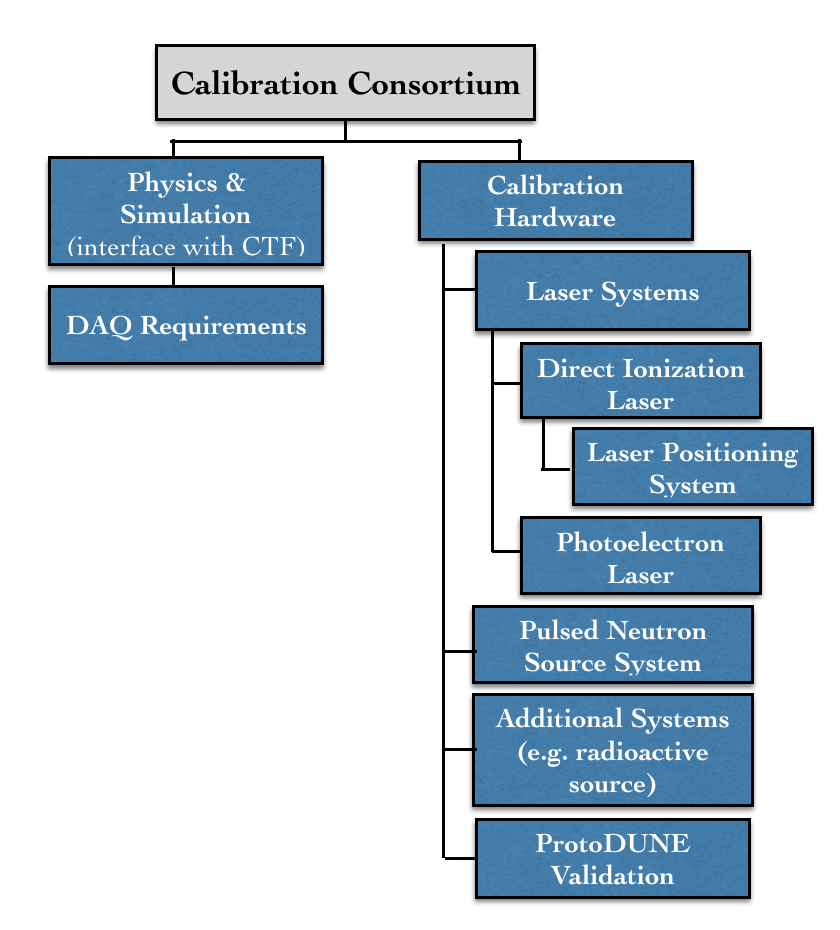
\includegraphics[height=4.0in]{graphics/calib_scope_chart.png}
\caption{Calibration consortium subsystem chart.}
\label{fig:scope_chart}
\end{figure}

%%%%%%%%%%%%%%%%%%%%%%%%%%%%
%\subsection{Requirements}
%\label{sec:sp-calib-ov-req}

%\input{vol-sp/ch-sp-calib-requirements}


%%%%%%%%%%%%%%%%%%%%%%%%%%%%
\subsection{Design Considerations and Requirements}
\label{sec:sp-calib-ov-consid}
%\fixme{SG, KM: Done; JM please check. }
%To-DO: Need more information on requirements from neutron source and RA source, once we have it, we can update the text/table as needed.}

Some common design considerations for calibration devices include stability, reliability, and longevity, so that calibration systems can be operated for the lifetime of the experiment (\dunelifetime). Such longevity is uncommon for any device, so the overall design allows replacement of devices where possible. The systems must also adhere to relevant global requirements of the DUNE detector; Table~\ref{tab:fdgen-calib-toplevel-reqs} shows the top-level requirements for calibration subsystems from the overall requirements. For example, DUNE requires the \efield  on any instrumentation devices inside the cryostat to be less than 30 kV/cm to minimize the risk of dielectric breakdown in \lar. A consideration important for event reconstruction is the maximum noise level induced by calibration devices that the readout electronics can tolerate. \dword{pdsp} is evaluating this. 

Table~\ref{tab:fdgen-calib-toplevel-reqs} \todo{This table was prepared manually not automatically generated; But, we have prepared the appropriate spreadsheet.} also shows the top-level requirements from each calibration subsystem. For the laser system, the energy and position reconstruction requirements for physics measurements lead to requirements on the necessary precision of the laser \efield measurement, its spatial coverage and granularity. The laser \efield measurement precision is required to be ~1\% so that the impact on the collected charge is well below 1\%. This is also motivated by consistency with the high level DUNE specification of 1\% on field uniformity throughout the volume due to component alignment and \hv system. For the laser coverage, in order to keep the \efield measurement precision at the ~1\% level, we aim to have a coverage of 75\% or better of the total fiducial volume (FV). The requirement on the granularity for laser is estimated based on the FV uncertainty requirements (1\%) and corresponding uncertainty requirements (1.5 cm) in each coordinate. A voxel size of \num{30}x\num{30}x\num{30}~cm is considered to be sufficient to satisfy the FV uncertainty requirements. 

The laser beam position is also required at the level of reconstruction requirement in each coordinate which is around 5~mm over 10 to 15~m where the latter is the distance between two consecutive laser ports in the beam direction. This results in a stringent requirement of 0.03$^{o}$ (or 0.5~mrad). The data volume for the ionization laser system is required to be at least 90~TB/year/10-kton assuming 800k laser pulses, \num{10}x\num{10}x\num{10}~cm voxel sizes, a 100~$\mu$s zero suppression window, and one dedicated calibration campaign per year.

For the pulsed neutron source system, the system must provide sufficient neutron event rate to make spatially separated precision measurements across the detector of comparable size to the voxels probed by the laser (\num{30}x\num{30}x\num{30}~cm) for most regions of the detector (75\%). For the supernova program, measurements from the PNS should demonstrate 1\% energy scale, 5\% energy resolution and 0.5 MeV detection threshold, and so each voxel should have sufficient neutron event rate to achieve this. %\todo{KM: Improve or remind connection to SN program? even though it's comparable? SG: maybe for 2nd draft?}
In terms of data volume requirements, the neutron source system requires about 84~TB/year/10-kton assuming 10$^{6}$ neutrons/pulse, 1000 neutron captures/m$^{3}$ and 1300 observed neutron captures per pulse and 6 calibration runs per year. 

For the proposed radioactive source system, it is important that the rate of the 9 MeV capture $\gamma$ events inside the source is less than 1~kHz so no more than one capture $\gamma$-event occurs during a single 2.2~ms drift period. 

Table~\ref{tab:fdgen-calib-all-reqs} shows the full set of requirements related to all of the calibration subsystems. More details on each of the requirements can be found under corresponding consortia.   
%\todo{Updated estimate for PNS DAQ rate to be added to Table 1.1 and 1.2}

\begin{dunetable}
[Specifications for calibration subsystems]
{p{0.45\linewidth}p{0.25\linewidth}p{0.25\linewidth}}
{tab:fdgen-calib-toplevel-reqs}
{List of top-level specifications for the different calibration subsystems. Global DUNE requirements are listed in bold.}  Quantity/Parameter	& Specification	& Goal		 \\ \toprowrule      
{\bf Noise from calibration devices}	 & $\ll$ 1000 enc   & \\ \colhline    
{\bf Max. \efield near calibration devices} & < 30 kV/cm & <15 kV/cm \\ \colhline     
Ionization Laser \efield measurement precision & 1\% & <1\% \\ \colhline
Ionization Laser \efield measurement coverage & > 75\% & 100\% \\ \colhline
Ionization Laser \efield measurement granularity & < \num{30}x\num{30}x\num{30}~cm & \num{10}x\num{10}x\num{10}~cm \\ \colhline
Laser beam position precision & 0.5 mrad & 0.5 mrad \\ \colhline
Neutron source coverage & > 75\% & 100\% \\ \colhline % neutron source
Ionization laser DAQ rate (per 10 kton) & 90~TB/year & 185~TB/year\\ \colhline
Neutron source DAQ rate (per 10~kton) & 84~TB/year & 168~TB/year\\ \colhline
Rate of 9~MeV capture $\gamma$-events inside the proposed radioactive source & < 1~kHz & \\ \colhline 
\end{dunetable}


\begin{dunetable}
[Specifications for calibration subsystems]
{p{0.45\linewidth}p{0.25\linewidth}p{0.25\linewidth}}
{tab:fdgen-calib-all-reqs}
{List of specifications for the different calibration subsystems}   
Quantity/Parameter	& Specification	& Goal		 \\ \toprowrule      

Noise from calibration devices	 & $\ll$ 1000 enc   & \\ \colhline    Max. \efield near calibration devices & < 30 kV/cm & <15 kV/cm \\ \colhline                     

\textbf{Direct Ionization Laser System} &    &   \\ \colhline   
\efield measurement precision & 1\% & <1\% \\ \colhline
\efield measurement coverage & > 75\% & 100\% \\ \colhline
\efield measurement granularity & < \num{30}x\num{30}x\num{30}~cm & \num{10}x\num{10}x\num{10}~cm \\ \colhline
Top field cage penetrations (alternative design) & to achieve desired laser coverage & \\ \colhline
DAQ rate per 10~kton & 90 TB/year & 185 TB/year \\ \colhline
Longevity	& \dunelifetime			& > \dunelifetime   \\ \colhline        
%Stability & Match precision requirement at all places/times	&  \\ \colhline  Reliability	& Measurements as needed & Measurements as needed \\ \colhline 
\textbf{Laser Positioning System} & & \\ \colhline                      
Laser beam position precision & 0.5~mrad & 0.5~mrad \\ \colhline
Longevity	& \dunelifetime			& > \dunelifetime   \\ \colhline        
%Stability & Match precision requirement at all places/times	&  \\ \colhline  Reliability	& Measurements as needed & Measurements as needed \\ \colhline    
\textbf{Photoelectron Laser System}	   &   &  \\ \colhline            
Longevity	& \dunelifetime			& > \dunelifetime   \\ \colhline        
%Stability & Match precision requirement at all places/times	&  \\ \colhline  Reliability	& Measurements as needed & Measurements as needed \\ \colhline

\textbf{Pulsed Neutron Source System}	   &   &  \\ \colhline        
Coverage & > 75\% & 100\% \\ \colhline
DAQ rate per 10~kton & 84~TB/year & 168~TB/year \\ \colhline 
Longevity	& 3 years			& \dunelifetime   \\ \colhline        
%Stability & Match precision requirement at all places/times	&  \\ 
%\colhline  Reliability	& Measurements as needed & Measurements as needed \\ \colhline

\textbf{Proposed Radioactive Source System}	   &   &  \\ \colhline  
Distance of the source from the field cage & 30 cm & \\ \colhline
Rate of 9~MeV capture $\gamma$-events inside the source & < 1kHz & \\ \colhline 
Data volume per 10~kton & 50~TB/year & 100~TB/year \\ \colhline 
Longevity	& \dunelifetime			& > \dunelifetime   \\ \colhline    
%Stability & Match precision requirement at all places/times	&  \\ \colhline  Reliability	& Measurements as needed & Measurements as needed \\ \colhline

\end{dunetable}


\subsubsection{Cryostat Configuration for Calibration}
\label{sec:calib-ports}
The current cryostat design for the %DUNE SP FD 
\spmod with penetrations for various sub-systems is shown in Figure~\ref{fig:ftmap}. The penetrations dedicated for calibrations are highlighted in black circles. The ports on far east and far west are located outside the field cage. The current plan is to use these penetrations for multiple purposes. For example, the penetrations on the far east and west will be used both by laser and radioactive source systems. In addition to these dedicated ports, the Detector Support System (DSS) and cryogenic ports (orange and blue dots in Figure~\ref{fig:ftmap}, respectively) will also be used as needed to route cables for calibration systems (e.g. the \dword{sp} \dword{pds}). There is plan to accommodate DSS and cryogenic ports with feedthroughs with a CF63 side flange for this purpose.   

\begin{figure}[tbp]
\centering
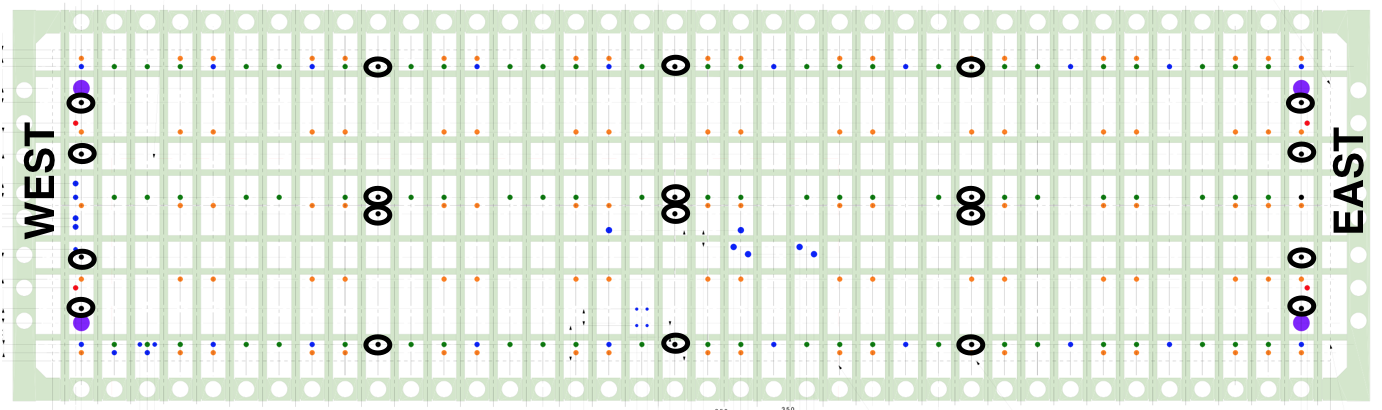
\includegraphics[height=2.0in]{FTmap.png}
\caption{Top view of the \spmod %DUNE SP FD 
cryostat showing various penetrations. Highlighted in black circles are multi-purpose calibration penetrations. The green dots are TPC signal cable penetrations. The blue ports are cryogenic ports. The orange ports are \dword{dss} penetrations. The larger purple ports at the four corners of the cryostat are human access ports.}
\label{fig:ftmap}
\end{figure}

The placement of these penetrations was largely driven by the ionization track laser %and radioactive source system 
requirements. The ports that are inwards of the cryostat are placed near the APAs (similarly to what is planned for SBND) to minimize any risks due to the HV discharge. For the far east and west ports, HV is not an issue as they are located outside the \dword{fc} and the penetrations are located near mid-drift (location favorable to possible source deployment).
%to meet radioactive source requirements. 
Implementation of the ionization track laser system proposed in Section~\ref{sec:sp-calib-sys-las-ion}, requires 20 feedthroughs to cover the four TPC drift volumes; this arrangement is needed for lasers to be used for full volume calibration of the E field and associated diagnostics (e.g. HV). 

The distance between any two consecutive feedthrough columns in Figure~\ref{fig:ftmap} is assumed to be about \SI{15}{\m}. This is considered reasonable since the experience from the \microboone laser system has shown that tracks will propagate over that detector's full \SI{10}{\m} length. Assuming that the effects of Rayleigh scattering and self-focusing (Kerr effect) do not limit the laser track length, this laser arrangement could illuminate the full volume with crossing track data.  It is important to note that at this point in time, a maximum usable track length is unknown and it is not excluded that the full \SI{60}{\m} \detmodule length could be achieved by the laser system after optimization.




%%%%%%%%%%%%%%%%%%%%%%%%%%%%%%%%%%%%%%%%%%%%%%%%%%%%%%%
%\cleardoublepage

\section{Calibration Systems}
\subsection{Laser Calibration Systems}
\label{sec:sp-calib-sys-las}

%\fixme{KM: Some of the "possible measurements" read more like development plans.}

%%%%%%%%%%%%%%%%%%%%%%%%%%%%
\subsubsection{Ionization Laser System}
\label{sec:sp-calib-sys-las-ion}

%%%%%%%%%%%%%%%
\subsubsubsection{Physics Motivation}
\label{sec:sp-calib-sys-las-ion-phys} 

%Adapted from IDR
The primary purpose of a laser system is to provide an independent, fine-grained estimate of the \efield in space and %changed or to and
time. 
Through its effect on drift velocity and recombination, the \efield is a critical parameter for physics signals as it ultimately impacts the spatial resolution and energy response of the detector.

 There are multiple sources which may distort the electric field temporally  or spatially in the detector. Current simulation studies indicate that positive ion accumulation and drift (space charge) due to ionization sources such as cosmic rays or ${}^{39}$Ar is small in the DUNE \dword{fd};  however, not enough is known yet about the fluid flow pattern in the FD to exclude the possibility of stable eddies which may amplify the effect for both \single and \dual modules. This effect can get further amplified significantly in the \dword{dpmod} due to ion accumulation at the liquid-gas interface. 
Additionally, other sources in the detector (especially detector imperfections) can cause \efield distortions. For example, field cage resistor failures, non-uniform resistivity in the voltage dividers, CPA misalignment, CPA structural deformations, and APA and CPA offsets and  deviations from flatness can create localized \efield distortions. 
In both SP and DP systems, the failure of a resistor will create significant, local electric field distortions which will need to be identified\footnote{In the DP system, four registers would have to fail to cause a failure across the field cage gap, but even one failure in the SP can have an impact; this may be partially mitigated by modifying the HV, but not completely.}. While the resistor failure will be detected temporally, its location in space is not possible to determine from monitoring data. Misalignments of detector objects or deformations may also create (small) electric field distortions; while individual effects may be small, it is possible to have a combined, significant effect.
Each individual \efield distortion may add in quadrature with other effects, and can reach 4\% under certain conditions. Understanding all these effects require in-situ measurement of \efield for proper calibration. 

Many useful secondary uses of laser include alignment (especially modes that are weakly constrained by cosmic rays),
%; see Figure~\ref{fig:apacurtainalign}),
stability monitoring, and diagnosing detector failures (e.g., \dword{hv}).  
Misalignment may include physical deformation and/or rotations of objects within the detector.  Certain alignment ``directions''  are difficult to assess with cosmic rays alone, such as distortions of the detector that preserve the gap widths and do not shift the \dwords{apa} in $x$ near the gaps relative to one another.
%are difficult to assess with cosmic rays alone. 
These distortions include global shifts and rotations in the locations of all detector elements, and crumpling modes where the edges of the \dwords{apa} hold together but angles are slightly different from nominal.   
%Addressed with (complementary) proposed laser and external muon tracking systems.

%% JM %% from early IDR version

A laser system also has the intrinsic advantage of
being immune to recombination, thus eliminating particle-dependent effects.  

%JM % from early IDR version. Now should go on PE laser section
%
%Even if the laser is not intense enough to ionize the \dword{lar}, electrons may be liberated from material on the cathode, which provides many useful measurements. The total drift time can be  assessed from laser pulse to readout of charge on the anode. A photo-electron-based calibration system was used in the T2K gaseous (predominantly Ar), TPCs~\cite{Abgrall:2010hi}. Targets placed on the cathode provided dots and lines that were then imaged by the electronics, and relative distortions of the surveyed positions could be used. The T2K photo-electron system provided measurements of adjacent electronics modules' relative timing response, drift velocity with few \si{\nano\s} resolution of \SI{870}{\milli\m} drift distance, electronics gain, transverse diffusion, and an integrated measurement of the electric field along the drift direction. For DUNE, the system would be similarly used as on T2K to diagnose electronics or TPC response issues on demand, and provide an integral field measurement and relative distortions of $y$, $z$ positions with time, and of either $x$ or drift velocity. Ejection of photo-electrons from the direct ionization laser system has also been observed.

%% JM %% end % from early IDR version

%%%%%%%%%%%%%%%

%JM % this should likely go in intro to both lasers.
%
%The Calibration task force has considered multiple systems that use a laser to extract the electric field map.  They fall into two categories: photo-electron and direct ionization of the \dword{lar}, both driven by a \SI{266}{\nano\m} laser system.

%Start by design requirements:
% size of voxels, crossing tracks

%\subsubsubsection{Requirements}
%\label{sec:laserReq}

%The energy and position reconstruction requirements for physics measurements lead to requirements on the necessary precision of the calibration \efield measurement and its spatial granularity.  

%As mentioned in the DUNE Physics TDR (Section 4.4.1.1), a \num{1}\% bias in the lepton energy scale is significant for the LBL sensitivity to CPV. Since a smaller \efield leads to higher electron/ion recombination and therefore a lower collected charge, distortions of the \efield are one of the possible causes of an energy scale bias.  According to \cite{mooney2018}, a \num{1}\% distortion on \efield leads to a \num{0.3}\% bias on collected charge.
%Since other effects will contribute to the lepton energy scale uncertainty budget, we consider a goal for the calibration system to measure the \efield to a precision of $\sim\num{1}\%$ so that its impact on the collected charge is well below \num{1}\%.

%The IDR states that a fiducial volume uncertainty of \num{1}\% is required (ref. \cite{idr-vol-1}, p. 4-46) and that this translates to a position uncertainty of \num{1.5}~cm in each coordinate (ref. \cite{idr-vol-2}, p. 2-12). Also that in the $y$ and $z$ coordinates, the wire pitch of \num{4.7}~mm  achieves that while in the drift ($x$) direction, the position is calculated from timing so it is claimed it should be known better.

%But the position uncertainty depends also on the electric field, via the drift velocity. Since the position distortions accumulate over the drift path of the electron, it is not enough to specify an uncertainty on the field, we must accompany it by specifying the size of the spatial region of that distortion. i.e. a \num{10}\% distortion would not be relevant if it was confined to a \num{2}~cm region, for instance, and the rest of the drift region was nominal. So what matters is the product of [size of region]x[distortion]. Moreover, we should distinguish distortions of two types:
%\begin{enumerate}
%\item affecting the magnitude of the field. Then the effect on the drift velocity $v$ is also a change of magnitude. According to the function provided in \cite{walkoviak2000}, close to \num{500}~V/cm, the variation of the velocity with the field is such that a \num{4}~\% variation in $E$ leads to a \num{1.5}~\% variation in $v$.
%\item 	affecting the direction of the field. Nominally, the field $E$ should be along $x$, so $E = E_L$ (the longitudinal component). If we consider that the distortions introduce a new transverse component $E_T$, in this case this translates directly into the same effect in the drift velocity, that gains a $v_T$ component that is $v_T=v_L  E_T/E_L $, i.e. a\num{4}~\% transverse distortion on the field leads to a \num{4}~\% transverse distortion on the drift velocity.
%\end{enumerate}

%So, a \num{1.5}~cm shift comes about from a constant \num{1.5}~\% distortion in the velocity field over a region of \num{1}~m. In terms of electric field, that could be from a \num{1.5}~\% distortion in ET over 1 m or a \num{4}~\% distortion in EL over the same distance.

%From ref. \cite{idr-vol-1}, page 4-53, \efield distortions can be caused by space-charge effects due to accumulation of positive ions caused by $^{39}$Ar decays (cosmic rate is low in FD), or detector defects, such as field cage resistor failures, resistivity disuniformities, etc... The total effects added in quadrature can be as high as \num{4}~\%. 
%From ref. \cite{mooney2018}, the space charge effects due to $^{39}$Ar can be of the order of \num{0.1}~\% for the single phase (SP), and \num{1}~\% for the dual phase (DP), so in practice that kind of distortion needs to cover several meters in order to be relevant.
%Other effects due to cathode plane assembly (CPA) or field cage (FC) imperfections can be higher than those due to space charge, but they are also much more localized. 
 %If we assume that there are no foreseeable effects that would distort the field more than \num{4}~\%, and considering the worst case (transverse distortions), then the smallest region that would produce a \num{1.5}~cm  shift is \num{1.5}/\num{0.04}~=~\num{37.5}~cm. That provides a target for the granularity of the measurement of the \efield distortions in $x$, with of course a larger region if the distortions are smaller. Given the above considerations, then a voxel size of \num{10}x\num{10}x\num{10}~cm appears to be enough to measure the \efield with the granularity needed for a good position reconstruction precision.
%In fact, since the effects that can likely cause bigger \efield distortions are the problems or alignments in the CPA (or APA), or in the FC, it could be conceivable to have different size voxels for different regions, saving the highest granularity of the probing for the walls/edges of the drift volume.

%%%%%%%%%%%%%%%%%%%%%%%%%%%%
\subsubsubsection{Requirements}
\label{sec:sp-calib-laser-req}


% KM outline
%% Requirements we are held to from other systems -- EB table -- see Jose's early talk
%% Targets for SN and LBL physics -- or just remind in other subsections? \fixme{KM: right now the targets for SN and LBL physics exist in the design sections.}
%% System must operate for a long time
    % SG: physics driven calibration requirements, need a table to connect calibration requirements to high level physics requirements, not easy, but we need to try

%\fixme{guidance coming soon!}

%\fixme{KM: adjusted to be specific to laser; SG: I have made some edits as well. JM: OK, signing off.}

%The DUNE physics requirements and the high level specifications of other existing systems are the driving motivation for the specifications of the performance of the dedicated calibration systems, described below. From those, and the constraints due to detector dimensions, etc, derive also the engineering specifications of each calibration system, described in each system's respective section.

%\paragraph{\efield measurements}
The energy and position reconstruction requirements for physics measurements lead to requirements on the necessary precision of the laser calibration \efield measurement, its spatial coverage and granularity. The next sections discuss the rationale behind each requirement, which we take as the DUNE specification.
%, with ALARA (or AHARA for the coverage) as goal.

\paragraph{\efield precision}

In the \dword{lbl} and high-energy range, the DUNE IDR states that ``...calibration information needs to provide approximately 1-2\% understanding of normalization, energy, and position resolution within the detector.'' (from \cite{idr-vol-1}, p. 4-47). 
The DUNE Physics TDR (Section 4.4.1.1) indicates that a \num{1}\% bias in the lepton energy scale is significant for the \dword{lbl} sensitivity to CPV.

Since a smaller \efield leads to higher electron/ion recombination and therefore a lower collected charge, distortions of the \efield are one of the possible causes of an energy scale bias. In order to connect that requirement to a specification on the necessary precision of the \efield measurement, we note that, via recombination studies\cite{mooney2018}, we expect a \num{1}\% distortion on \efield to lead to a \num{0.3}\% bias on collected charge.

Since other effects will contribute to the lepton energy scale uncertainty budget, we consider a goal for the calibration system to measure the \efield to a precision of $\sim\num{1}\%$ so that its impact on the collected charge is well below \num{1}\%.
This is also motivated by consistency with the high level DUNE specification on field uniformity throughout the volume due to component alignment and HV system, that was set at \num{1}\%.

Together with two other high-level DUNE specifications, the APA wire spacing (4.7~mm) and the front end peaking time (1~$\mu s$), the impact of this \efield precision requirement on engineering parameters of the calibration laser system is discussed further ahead, in Section \ref{sec:sp-calib-sys-las-ion-meas}.

\paragraph{\efield measurement coverage}

In practice, measuring the \efield  ~``throughout the [whole] volume'' of the TPC will be difficult, 
%hard, 
so we must establish a goal for the coverage and granularity of the measurement. 
Until a detailed study of the propagation of the coverage and granularity into a resolution metric is available, we can already make a rough estimation of the necessary coverage in the following way. Taking \num{4}\% as the maximum \efield distortion resulting from a compounding of multiple possible effects in the DUNE FD (\cite{idr-vol-1}, page~4-53), we can then ask what would be the maximum acceptable size of the spatial region uncovered by the calibration system, if a distortion of that magnitude (systematically biased in the same direction) were present. In order to keep the overall (average) \efield distortion at the \num{1}\% level, then that region should be no larger than \num{25}\% of the total fiducial volume. Therefore, we aim to have a coverage of \num{75}\% or better.

\paragraph{\efield measurement granularity}

The IDR states that a fiducial volume uncertainty of \num{1}\% is required (ref.~\cite{idr-vol-1}, p.~4-46) and that this translates to a position uncertainty of \num{1.5}~cm in each coordinate (ref.~\cite{idr-vol-2}, p.~2-12). Also that in the $y$ and $z$ coordinates, the wire pitch of \num{4.7}~mm achieves that while in the drift ($x$) direction, the position is calculated from timing so it is claimed it should be known better.

But the position uncertainty depends also on the electric field, via the drift velocity. Since the position distortions accumulate over the drift path of the electron, it is not enough to specify an uncertainty on the field, we must accompany it by specifying the size of the spatial region of that distortion. i.e. a \num{10}\% distortion would not be relevant if it was confined to a \num{2}~cm region, for instance, and the rest of the drift region was nominal. So what matters is the product of [size of region] $\times$ [distortion]. Moreover, we should distinguish distortions of two types:
\begin{enumerate}
\item those affecting the magnitude of the field. Then the effect on the drift velocity $v$ is also a change of magnitude. According to the function provided in \cite{walkoviak2000}, close to \num{500}~V/cm, the variation of the velocity with the field is such that a \num{4}~\% variation in $E$ leads to a \num{1.5}~\% variation in $v$.
\item those affecting the direction of the field. Nominally, the field $E$ should be along $x$, so $E = E_L$ (the longitudinal component). If we consider that the distortions introduce a new transverse component $E_T$, in this case this translates directly into the same effect in the drift velocity, that gains a $v_T$ component that is $v_T=v_L  E_T/E_L $, i.e. a \num{4}~\% transverse distortion on the field leads to a \num{4}~\% transverse distortion on the drift velocity.
\end{enumerate}

So, a \num{1.5}~cm shift comes about from a constant \num{1.5}~\% distortion in the velocity field over a region of \num{1}~m. In terms of electric field, that could be from a \num{1.5}~\% distortion in $E_T$ over 1~m or a \num{4}~\% distortion in $E_L$ over the same distance.

From ref.~\cite{idr-vol-1}, page~4-53, \efield distortions can be caused by space-charge effects due to accumulation of positive ions caused by $^{39}$Ar decays (cosmic rate is low in FD), or detector defects, such as field cage resistor failures, resistivity non-uniformities, etc. These effects added in quadrature can be as high as \num{4}~\%. From ref. ~\cite{mooney2018}, the space charge effects due to $^{39}$Ar can be of the order of \num{0.1}~\% for the single phase (SP), and \num{1}~\% for the dual phase (DP), so in practice these level of 
%that kind of distortion 
distortions need to cover several meters in order to be relevant.
Other effects due to \dword{cpa} or \dword{fc} imperfections can be higher than those due to space charge, but they are also much more localized. If we assume that there are no foreseeable effects that would distort the field more than \num{4}~\%, and considering the worst case (transverse distortions), then the smallest region that would produce a \num{1.5}~cm  shift is \num{1.5}/\num{0.04}~=~\num{37.5}~cm. This provides a target for the granularity of the measurement of the \efield distortions in $x$ to be smaller than about \num{30}~cm, with of course a larger region if the distortions are smaller. Given the above considerations, then a voxel size of \num{10}x\num{10}x\num{10}~cm appears to be enough to measure the \efield with the granularity needed for a good position reconstruction precision. In fact, since the effects that can likely cause bigger \efield distortions are the problems or alignments in the CPA (or APA), or in the FC, it could be conceivable to have different size voxels for different regions, saving the highest granularity of the probing for the walls/edges of the drift volume.

\begin{comment}
\begin{dunetable}
[Calibration Requirements]
{p{0.5\textwidth}p{0.15\textwidth}p{0.15\textwidth}}
{tab:calibreq}
{Calibration Specifications and Goals}   
Requirement & Specification & Goal \\ \toprowrule
\efield measurement precision & < 1\% & ALARA \\ \colhline
\efield measurement coverage & > 75\% & AHARA \\ \colhline
\efield measurement granularity & < 30x30x30 cm & ALARA \\ \colhline
\end{dunetable}
\end{comment}



\subsubsubsection{Design}
\label{sec:sp-calib-sys-las-ion-des}

\paragraph{Baseline design}

The design of the laser calibration system for DUNE is strongly based on the design of the system built for \dword{microboone} ~\cite{microboone}, that was based on several previous developments~\cite{rossi2009,Zeller:2013sva,ereditato2014,Ereditato:2014tya}. A similar system was also built for CAPTAIN~\cite{captain-wp} and in the near future, will be built for SBND~\cite{sbn-prop}. Operation of the \dword{microboone} system has already taken place and a preliminary report was given in~\cite{chen2018}.

Ionization of \dword{lar} by laser can occur via a multiphoton process in which a two-photon absorption~\cite{badhrees2010} leads the atom to the excited states band, and a third photon can cause ionization. This can only occur with high photon fluxes, and so the employed lasers need to be pulsed and have pulse energies of \num{60}~mJ or more. Contrary to muons, the laser beams do not suffer multiple scattering and travel along straight lines determined by the steering mirror optics. The basic measurement consists in recording the laser beams with the TPC and comparing the reconstructed tracks with the direction known from the steering hardware. An apparent curvature of the measured track is attributed to \efield distortions (either in direction or magnitude).

An unambiguous field map requires crossing laser tracks in every relevant "voxel" of the detector. If two tracks that enter the same spatial voxel ($10 \times 10 \times 10 ~\textrm{cm}^3$ volume) in the \dword{detmodule}, the relative position of the tracks provides an estimate of the local \threed \efield.

With a single, steerable laser track, there would be ambiguity in the direction/magnitude of the position displacement and so the information obtained would be limited. Even if not crossing, a set of several tracks from opposite directions can still be used to obtain a displacement map via an iterative procedure~\cite{chen2018}.

%The laser track location placement precision is limited solely by the optics design and self-focusing effects can impact the practical range of the track (theoretically, the Rayleigh scattering length of 266~nm light is about 40~m). As discussed in Section~\ref{sec:FTs}, this is mitigated by spacing lasers about 15~m apart which is very close to the laser track range demonstrated by the MicroBooNE experiment. 
 
%\fixme{Clarify the extra degeneracy in this case, related to overall parameterization of TPC response model?}
%\fixme{Need to reference optics of system?}

%\fixme{Add a comment on how long a run takes} 

%A \phel{}-based calibration system was used in the T2K gaseous (predominantly Ar), TPCs~\cite{Abgrall:2010hi}. %Targets placed on the cathode provided dots and lines that were then imaged by the electronics, and relative distortions of the surveyed positions could be used. 
%Thin metal surfaces placed at surveyed positions on the cathode provided point-like and line sources of \phel{}s when illuminated by a laser. The T2K \phel system provided measurements of adjacent electronics modules' relative timing response, drift velocity with few \si{\nano\s} resolution of \SI{870}{\milli\m} drift distance, electronics gain, transverse diffusion, and an integrated measurement of the electric field along the drift direction. For DUNE, the system would be similarly used as on T2K to diagnose electronics or TPC response issues on demand, and provide an integral field measurement and relative distortions of $y$, $z$ positions with time, and of either $x$ or drift velocity. Ejection of \phel{}s from the direct ionization laser system has also been observed, so it is likely this is a reasonable addition to the nominal design.% and would only be considered a primary system if the intensity of the laser is problematic. 

%% JM %% from early IDR version


% Mini workshop: https://indico.fnal.gov/event/14909/

Laser beams with lengths of \num{10}~m in \dword{lar} have been observed in \dword{microboone}, and beams with \num{20}~m (possibly more) are reasonably expected to be possible to obtain with a similar system. While the Rayleigh scattering of the laser light is about \SI{40}{\m}, additional optics effects, including self-focusing (Kerr) effects may limit the maximum practical range.
This has determined the choice of locating 5 calibration ports in the cryostat roof at \num{15}~m intervals along each of the 4 drift volumes of the SP module, for a total of 20 ports. In fact, there are 4 ports just outside each of the FC end-walls, and 12 ports located over the top FC, close to the APA of each drift volume, as shown in Fig. \ref{fig:ftmap}.


\begin{figure}[htb!] 
\centering 
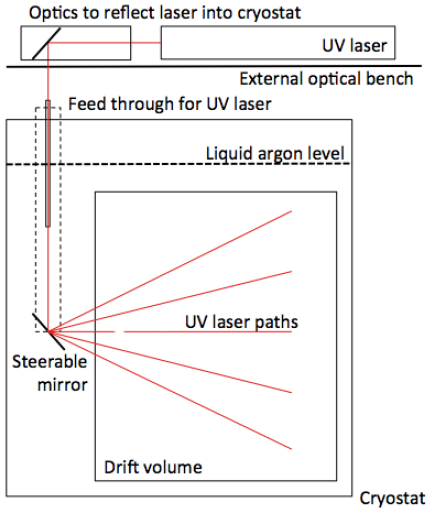
\includegraphics[width=0.45\linewidth]{graphics/uB_laser_schematic.png}
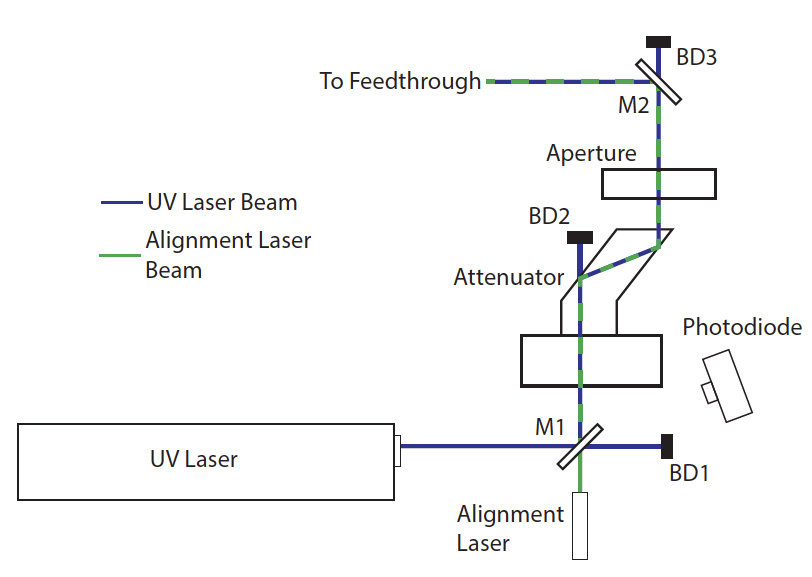
\includegraphics[width=0.5\linewidth]{graphics/uB_laser_box.png}
\caption{Left: Schematics of the ionization laser system in one port (from\cite{sbn-prop}). Right: Schematics of the laser box (from\cite{microboone}).}
\label{fig:laser_schematic} 
\end{figure} 


For each of those 20 ports, a laser module can be schematically represented by Fig. \ref{fig:laser_schematic} (Left), and consists of the following elements:
\begin{itemize}
    \item a laser box Fig. \ref{fig:laser_schematic} (Right) that provides:
    \begin{itemize}
        \item an attenuator and a collimator to control the intensity and size of the beam;
        \item a photodiode that gives a TPC-independent trigger signal;
        \item a low-power red laser, aligned with the UV one, to facilitate alignment operations;
        \item a Faraday cage to shield the surrounding electronics from the accompanying EM pulse.
    \end{itemize}
    \item a feedthrough (Fig. \ref{fig:laser_cad} (Left)) into the cryostat that provides:
    \begin{itemize}
        \item the optical coupling that allows the UV light to pass through into the cryostat directly into the liquid phase, avoiding distortions due to the gas-liquid interface and the gas itself;
        \item a rotational coupling that allows the whole structure to rotate while maintaining the cryostat seal;
        \item a periscope structure (Fig.~\ref{fig:laser_cad} (Right)) mounted under that rotating coupling, that supports a mirror within the \dword{lar};
        \item the additional theta rotation of the mirror is accomplished by a precision mechanism coupled to an external linear actuator;
        \item both the rotation and linear movements of the steering mechanism are read-out by precision encoders.
    \end{itemize}
    
\end{itemize}

\begin{figure}[htb!] 
\centering 
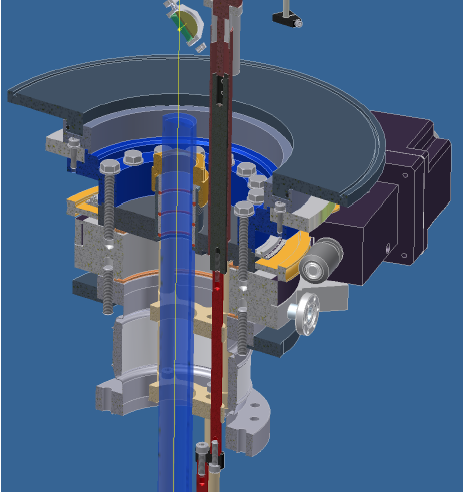
\includegraphics[width=0.49\linewidth]{graphics/uB_laser_ft.png}
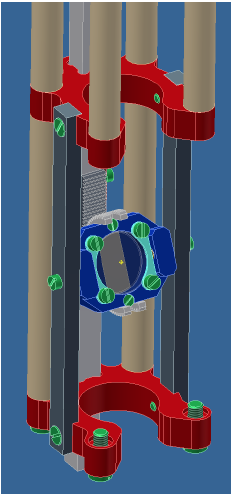
\includegraphics[width=0.248\linewidth]{graphics/uB_laser_periscope.png}
\caption{Left: CAD drawing of the \dword{microboone} feedthrough. Right: CAD drawing of the \dword{microboone} periscope. Both figures from\cite{microboone}.}
\label{fig:laser_cad} 
\end{figure} 

In the case of the lasers in the end-wall ports, the beams enter the FC laterally, while in the case of the lasers in the ports over the TPC, the beams enter the TPC from the top. In both cases, the laser beam can enter the FC only through the gaps between the FC electrodes. These gaps are \num{1.4}~cm wide and the electrodes themselves are \num{4.6}~cm wide, so it's clear that the shadowed regions are very significant. In one of the alternative designs, the top FC is modified as to allow small openings for the bottom of the periscope to penetrate within the FC, significantly increasing coverage.

For the six most central ports, the distance between them is small enough that we can consider having the same laser box serving two feedthroughs, in order to reduce the costs associated with the laser and its optics.

%a \SI{266}{\nano\m} laser would be mounted on the top of the cryostat, and service two adjacent feedthroughs. A steerable head and fiber interface would be mounted in the feedthrough, which is coated in a insulator. Two options are under investigation: (1) the \dword{fc} (but not the \dword{gp}) is penetrated, and (2) the \dword{fc} is not penetrated. In the former case, the \dword{fc} penetration has been shown to create a small distortion to the E-field, for the benefit of full volume E-field mapping. When the \dword{fc} is not penetrated, the laser shines through the \dword{fc} tubes, producing some regions that are not mappable by the laser. Unlike the ports that are inwards of the cryostat, the lasers through penetrations that are outside the \dword{fc} on the far east and west side of the cryostat will not penetrate the field cage. The photo-electron system would include a fiber and no steering; the necessity of penetrating the \dword{fc} is unlikely but has not been assessed yet.

A scan of the full detector using \SI{1}{L} volume elements would require a number of tracks on the order of 800k, would take about three days. It is expected that shorter runs could be done to investigate specific regions. The sampling granularity, and therefore the amount of data taken, is dependent on \dword{daq} requirements. In fact, even to be able to record the desired 800k tracks, a dedicated data reduction algorithm will have to be devised, so that only a drift window of about $100 \mu s$ of data is recorded, and the position of that window depends on the beam position and direction and which wire is being read out. More details on this are given in section~\ref{sec:sp-calib-daqreq}.

%The direct ionizing laser system may also be used to create \phel{}s from the cathode, even under low power operation.

%% JM %% end % from early IDR version

\paragraph{Alternative design 1: Top \dword{fc} penetration}

Given that the FC electrodes are 4.6~cm wide with only a small 1.4~cm gap between them, the shadows caused when the laser source is outside the FC are substantial. We estimate that the maximum angle at which beams can go through is about 45$^{o}$. Given the limitations of the region above the FC, especially the geometry of the ground plane, it is likely that the mirror cannot be placed much higher up than 40~cm away from the FC. That means that, close to the top FC, the covered region will be only about 40-60~cm long, in each 3.6~m long drift volume. Considering for simplicity no limitations to movement along the direction of the FC electrodes, that means that only about 10-15\% of the top area of the FC would be covered by the laser system. On the bottom FC, that ratio would be slightly higher, corresponding to the ratio of gap (1.4~cm) to total (1.4+4.6~cm) width, i.e. about 25\%.

Penetration of the FC would eliminate those shadows and allow a practically unimpeded coverage. Fig.~\ref{fig:laser_intofc} shows a possible way to accomplish this for the top-of-TPC ports. In practice, it might be necessary to remove two FC electrodes, to achieve a 10~cm diameter free circle. 

\begin{figure}[htb!] 
\centering 
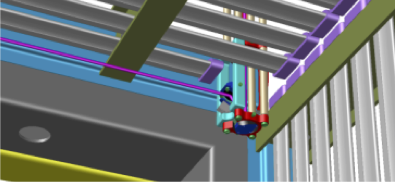
\includegraphics[width=0.8\linewidth]{graphics/dune_laser_sbndstyle.png}
\caption{CAD drawing of a possible way for the periscope to penetrate the FC.}
\label{fig:laser_intofc} 
\end{figure} 

In the end-walls, such a solution is more complicated
%not possible 
since the ports are on the side, not on top of the FC. Alternative 2 in the next section addresses the coverage issues with that design.

\paragraph{Alternative design 2: End-wall horizontal track}

The baseline design is based on laser entry points in which the movement of the steering mirror has two angular degrees of freedom.
 
A possible alternative design would change that end part of the system so that there is a translation and a rotation movement. A mirror at a \num{45}$^{o}$ angle would send the beam horizontally, perpendicular to the APA/CPA, but externally to the field cage. A horizontal track, installed in that same direction, would allow the translation movement of a secondary mirror (or two of them, one on each side), mounted with an angle of \num{45}$^{o}$ with respect to the incident beam. This allows the mirror to be aligned with the \num{1.4}~cm wide gaps between the field cage profiles. This second mirror would have a rotation movement, around the same axis, keeping the \num{45}$^{o}$ angle to the beam, but causing its reflection to sweep a vertical plane. Figure~\ref{fig:laser_alter2} provides an illustration of the mirror movements in this arrangement.

\begin{figure}[htb!] 
\centering 
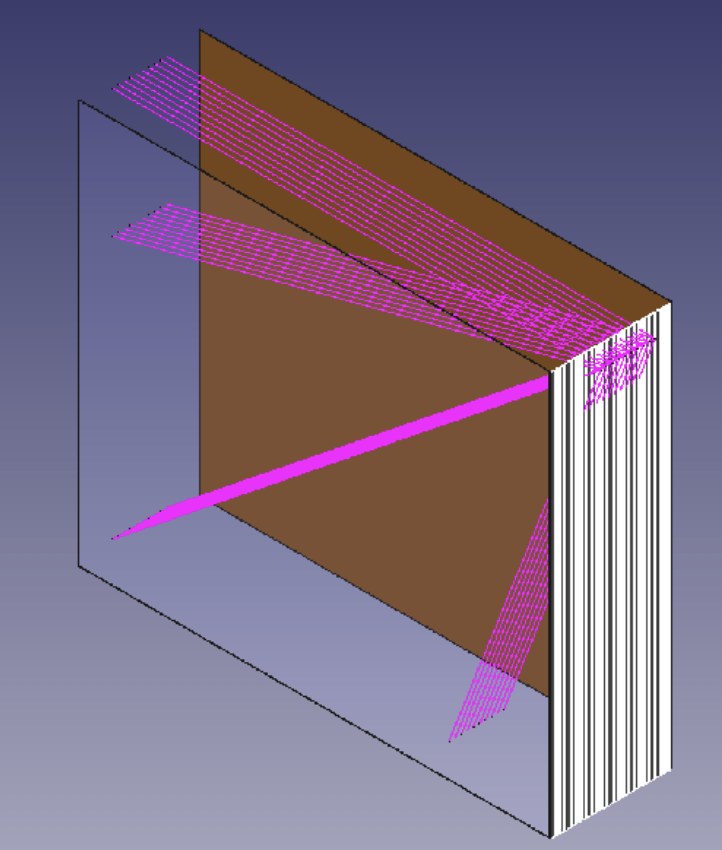
\includegraphics[width=0.5\linewidth]{graphics/Laser_alternative2.png}
\caption{Sketch of the beam array using end-wall horizontal track arrangement. The two planes on either side of the laser tracks (magenta) are cathode and anode.}
\label{fig:laser_alter2} 
\end{figure} 

In terms of cryostat penetration, the design of the feedthrough and periscope would follow the baseline one, but the $\theta$ angle would be practically always num{45}$^{o}$, with only minor adjustments, and the angle would flip between 0$^{o}$ and 180$^{o}$. 
%ref Newport mirror for 266 nm, https://www.newport.com/p/10QM20HM.75
The reflected beam is parallel to the FC wall and perpendicular to the APA. There would have to be a new \num{14}~m long tray for the movement of the secondary mirror(s). 
Long plastic threaded rods could be used for the movement along the tray. Rotation of the first rod would push/pull a small platform along the tray, and the rotation of the second rod is transmitted to a mechanism on that platform to achieve the rotation around the $x$ axis.

The FC profiles are 4.6~cm wide with a 1.4~cm gap between. That's the gap close to which the mirror needs to stop. That means that there is a finite amount of $x$ values where we can position the mirror, effectively every 6~cm. In order to correct for possible FC shifts, one can use the laser positioning system to see if beam is passing to the other side. Choosing the $z$ coordinate of the tray to be located close to an edge of the drift volume, the angular range of movement needed to fully cover a vertical plane with the rotation of the mirror is only 90$^{o}$.

The advantages of this mirror movement system are the following:
\begin{itemize}
\item should allow a good coverage of most of the TPC active volume, even coming from outside the FC;
\item one can use the same calibration port laser to illuminate all drift volumes;
\item the beam is always parallel to the APA, especially the PDS, so has less risk of hitting it directly or through reflections on the cathode (but by reflections on the FC electrodes, that's still possible);
% * <maneira@gmail.com> 2018-10-22T07:07:38.035Z:
% 
% is there any calculation of the space charge effect of the laser beams themselves? the number of tracks we want to use is pretty high.
% 
% ^.
\end{itemize}

With respect to the reference system, possible disadvantages are the following:
\begin{itemize}
\item in terms of construction, this option has more moving parts and movement transmitted at long distances, so it can be more challenging to reach the same kind of mechanical precision as the baseline one;
\item if the field cage profiles shift during cooling, there will be the need to fine-tune the alignment of the mirror with the FC gaps. This could be accomplished with the laser positioning system described in section~\ref{sec:calib-laser-pos};
%% JM %% include Jelena's text about it and reference it here.
 
\end{itemize}


%%%%%%%%%%%%%%%
\subsubsubsection{Possible Measurements}
\label{sec:sp-calib-sys-las-ion-meas}


The method for \efield measurement is based on the measurement of position displacements. The laser produces straight tracks in a known position and deviations from that seen in reconstructed tracks are attributed to \efield distortions. Therefore the precision with which the \efield distortions can be measured depends on the precision with which we can know the laser track position and the TPC position reconstruction precision.
The TPC precision is given primarily by the wire spacing of 4.7~mm in the $y$, $z$ coordinates and slightly better than that (maybe 2~mm) on the $z$ coordinate, determined by the $1~\mu s$ peaking time of the electronics. Given infinite laser positioning accuracy, the smallest measurable \efield distortions would be those that cause displacements of this magnitude --- 2 mm in $x$ and 5 mm in $y$, $z$. The precision on the drift velocity distortions depends on the size of the spatial region where they are present. For distortions present in regions of 0.5~m and larger, drift velocity distortions can therefore be measured with an accuracy of 1\% in $y$, $z$ and 0.4\% in $x$. In $y$, $z$, 1\% precision on drift velocity distortions translates to a 1\% precision on the transverse field distortions. Along $x$, one must consider that, at 500 V/cm, a 1\% change in \efield leads to 0.375 \% change in drift velocity. Therefore finally, this means that the smallest measurable distortions given the TPC design (wire pitch, timing precision) are of 1\% in \efield if they are present in regions of 0.5~m and above (smaller field distortions could be in principle be measurable if they are present over larger regions, so that their effect accumulates over the drift path).
On one side, this gives us an ultimate limit to the \efield precision achievable with the laser system, but on the other side, since these TPC precision considerations apply to physics events too, it also tells us that an \efield precision much better than 1\% should not have an impact on physics.

In principle, if we were confident about the field in one detector region and would like to probe another, we could use tracks that cross both regions and use the TPC measurements in the ''good'' region as the ``true'' track direction, without needing the hardware information on the mirror angles, etc. But in a general case, the TPC precision is only one of the components of the laser measurement precision, the other being the mechanical beam positioning accuracy. The goal of the mechanical design of the system is to achieve a precision close to that of the TPC measurements, so that no single factor is dominant in the overall systematics. The starting point of the laser beams is given by the position of the mirror in the periscope, that is known from construction drawings and cool down calculations. Warm surveys might be necessary. The angle of the beam is given by the angles ($\theta$, $\phi$) of the mirror, that are set by the periscope motors and read-out by the encoders. 
Reference~\cite{chen2018} quotes a mechanical precision of 0.05 ~mrad for the \dword{microboone} system, for both angles. At 10~m, the maximum distance in \dword{microboone}, that's 0.5~mm. In DUNE, we count on having 20~m long beams, so the precision is 1~mm at that distance, if we equal the precision of the \dword{microboone} system. The beam itself is wider than that. In fact, with a 0.5~mrad divergence, we expect the beam to be 1~cm wide at 20~m. The profile is Gaussian, so the centroid of the charge creation should be more accurate. During cool down, there can be shifts that need to be measured and corrected for, so we aim to have a system that can measure the beam position in a few positions, at least one per drift volume and laser beam. Our goal is to provide the position of the beam to an accuracy of 5~mm with positioning systems located at about 10~m from the beam origin.



 
 %% JM %% discuss how to get the \efield from the measurements even if the absolute knowledge of the laser track is not perfect.
 % - need for crossing tracks
 % - use positioning system
 % - do relative measurements between tracks close by. actual advantage of the alternative system: many parallel tracks at different x
 
 % also, estimate time needed and discuss idea of having the photo-laser for a quick/rough monitoring, and the ionization laser as a detailed probe of regions identified as possibly problematic.


%The remaining studies for the laser systems to be done prior to the \dword{tdr} are: 
%\begin{itemize}
%\item Determine a nominal design for photoelectric thin metal surfaces on the cathode. A survey in cold conditions is not possible for the \single system, and the photoelectric system could provide both known positions in the detector and information complementary to a survey or cosmic data.
%\item For the \dual system, quantify the additional benefit of a photoejection system since it will be possible to survey the \dwords{crp} externally under cold conditions.
%\item  Determine whether the known classes of possible \efield distortions warrant a mechanical penetration of the \dword{fc} (versus reduced sampling from projecting laser light inward between \dword{fc} elements) and further understand sensitivity of the laser to realistic \efield distortions. 
%\item Continue to study the range of possible \efield distortions in order to further refine the estimation of overall variation of the \efield  in the \dword{detmodule}. 
%\end{itemize}
%\begin{itemize}
%\item Determine  a nominal design for photoelectric targets on the cathode, and whether  such targets would provide sufficient survey-like information.
%\item Determine if the known classes of possible \efield distortions require penetration of the \dword{fc} (versus reduced sampling from shining between the field cage). 
%\item Further understand limitations on laser location precision, practical range of propagation due to optics design and Rayleigh scattering. \fixme{KM: Is this too vague to be helpful or sets us up for failure? What specifically will be studied?}
%\item Continue to quantify the range of possible \efield distortions in the DUNE FD to further refine the estimation of overall variation of \efield (both locally and globally) in the detector.
%\end{itemize}

%\fixme{}




\subsubsubsection{Laser positioning system}
\label{sec:calib-laser-pos}
\paragraph{Physics Motivation}

While the direction of the laser beam will be very well known based on the reading from the encoders on the laser beam steering mechanism,  residual uncertainty or unpredictable shift in the pointing direction will remain. Having in mind long length of the ionization track of more than 15\,m, even a small offset in the pointing direction can lead to vastly different ionization track location, especially close to the end of
the track. Such inaccuracies will directly impact the ability to precisely calibrate any variations in the \efield.

\paragraph{Design}

Laser positioning system (LPS) is designed to address the problem of precise and accurate knowledge of the laser track coordinates. %University of Hawaii group has 
Such a system (consisting of 1$\times$3) array was built for the miniCAPTAIN experiment and installed version is visible in the photo of the miniCAPTAIN TPC Fig.~\ref{fig:miniCAPTAIN}.  
\begin{figure}[htb!] 
\centering 
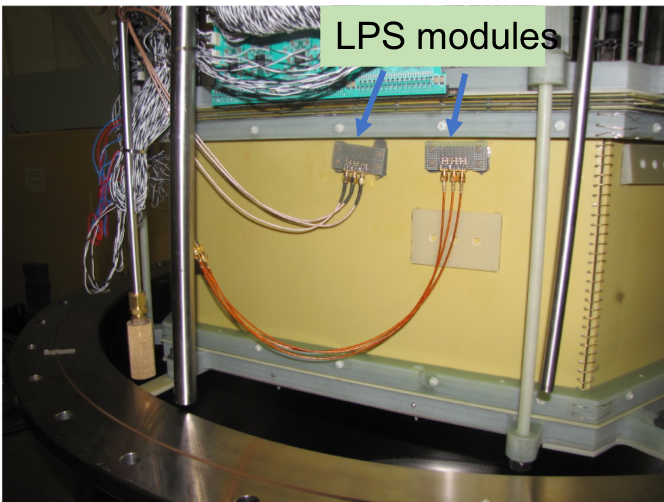
\includegraphics[width=0.6\linewidth]{LPS_miniCAPTAINlabeled.png} 
\caption{Photo of the miniCAPTAIN TPC with two LPS modules glued on the outside, in order to detect laser beam spot location via fluorescence of the TPC FR4 wall when illuminated by the laser beam.}
\label{fig:miniCAPTAIN} 
\end{figure}
LPS consists of groups of 9 pin diodes, operating in passive, photovoltaic mode. These are GaP diodes whose sensitivity range extends down to 200\,nm wavelength --- thus detecting 266\,nm light is straightforward. Fig.~\ref{fig:LPS1} and Fig.~\ref{fig:LPS2}  show signal detected at room and cryogenic
temperatures. PIN diode was illuminated by the 266\,nm light from the NdYag
laser in the lab 
%(in the lab at University of Hawaii) 
set at lowest possible setting for minimal power. Pin diode pads receive light via optical fiber bundles that are mounted on the opposite side from the laser injection points to eliminate issues with field cage interference. Drawings of one such group of pin diodes is shown in Figs.~\ref{fig:pin1} and Fig.~\ref{fig:pin2}. With the group of 9 photodiodes, one cannot only detect the beam but also crudely characterize its profile, giving a more precise location of the central beam pulse axis.


%\begin{figure}[htb!] 
%\begin{minipage}[b]{0.47\textwidth}
%\centering 
%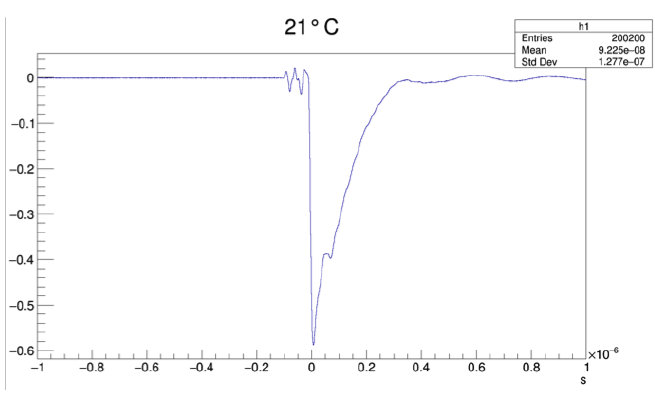
\includegraphics[width=0.95\linewidth]{GaP_diode_room_temp.png} 
%\caption{Signal from the GaP pin diode. The signal was a result of illumination of the PIN diode face with a 266\,nm laser at room temperature.}
%\label{fig:LPS1} 
%\end{figure}
%\end{minipage}
%\hfill
%\begin{minipage}[b]{0.47\textwidth}
%\begin{figure}[htb!] 
%\centering 
%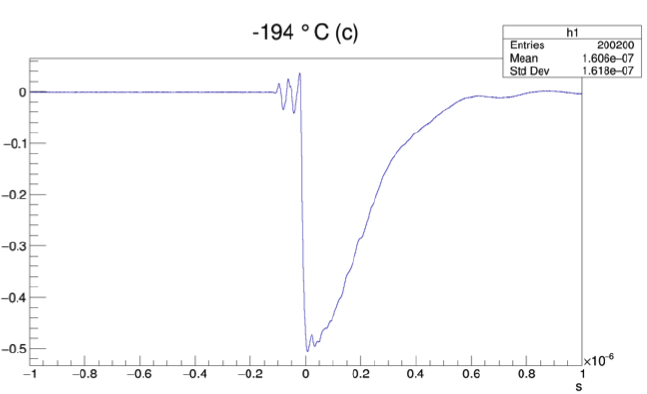
\includegraphics[width=0.95\linewidth]{GaP_diode_cryo_temp.png} 
%\caption{Signal from the GaP pin diode. The signal was result of illumination of the PIN diode face with a 266\,nm laser at cryogenic temperature.}
%\label{fig:LPS2} 
%\end{minipage}
%\hfill
%\end{figure} 


\begin{figure}[htb!] 
\begin{minipage}[b]{0.47\textwidth}
\centering 
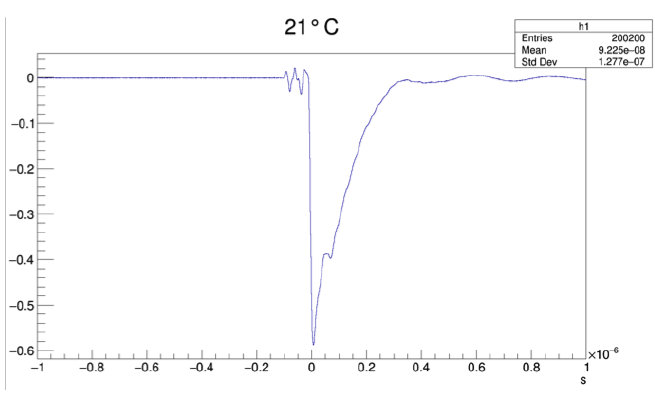
\includegraphics[width=1.0\linewidth]{GaP_diode_room_temp.png} 
\caption{Signal from the GaP pin diode. The signal was a result of illumination of the PIN diode face with a 266\,nm laser at room temperature.}
\label{fig:LPS1} 
\end{minipage}
\hfill
\begin{minipage}[b]{0.47\textwidth}
\centering 
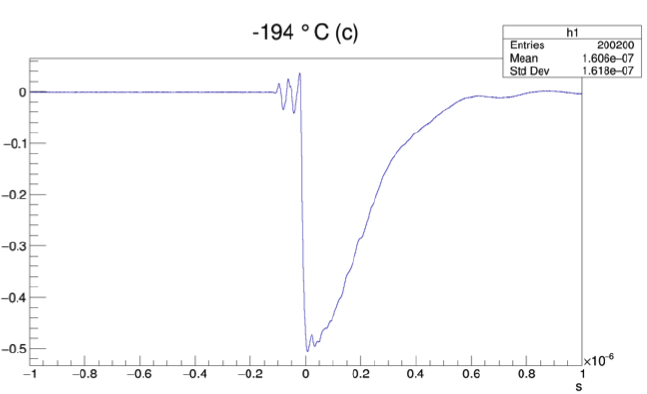
\includegraphics[width=1.0\linewidth]{GaP_diode_cryo_temp.png} 
\caption{Signal from the GaP pin diode. The signal was result of illumination of the PIN diode face with a 266\,nm laser at cryogenic temperature.}
\label{fig:LPS2} 
\end{minipage}
\hfill
\end{figure} 

\begin{figure}[htb!] 
\begin{minipage}[b]{0.4\textwidth}
\centering 
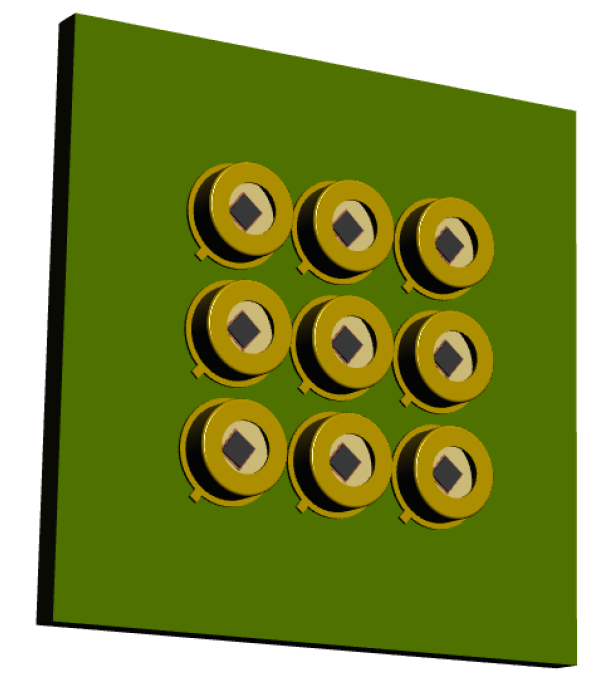
\includegraphics[width=0.95\linewidth]{GaP_assembly.png} 
\caption{LPS cluster that is mounted on the opposite wall from the laser periscope to detect and accurately determine the end point of the laser beam.}
\label{fig:pin1} 
\end{minipage}
\hfill
\begin{minipage}[b]{0.47\textwidth}
\centering 
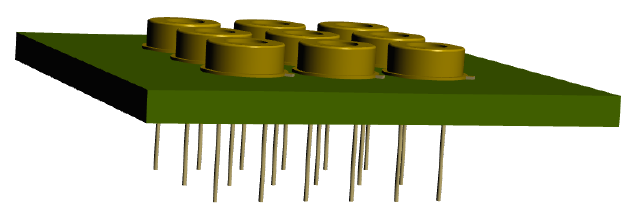
\includegraphics[width=0.95\linewidth]{GaP_assembly_profile.png} 
\caption{Profile of the LPS group mounted on the PCB. GaP diodes come with pins that utilize twisted pair to transport the signal.}
\label{fig:pin2} 
\end{minipage}
\hfill
\end{figure} 

There will be one LPS pad per laser. Laser would always send the first pulse in the direction of the LPS before proceeding into a calibration sequence.
 The electronics used to collect
signals from the LPS will be provided by the slow control group.

\paragraph{Possible measurements}
The utilization of the fiber bundle to deliver the 266\,nm photons to LPS needs to be verified in the lab. Lab measurements are currently underway to measure light attenuation in the fiber bundles (that go to the GaP diodes) as a function of fiber diameter and length. Further optimization of the LPS assembly to reduce electronic noise and cross-talk is required, among other things. Another important aspect is durability of the system that will require extensive running in the cryogenic conditions with  a large number of cool-downs to validate GaP for extended use in DUNE. Finally, alternatives to GaP such as SiPMs are under consideration. While SiPMs require power, their sensitivity to single photons makes them a desirable candidate for low light signals. 

%\fixme{KM: I think I got the number of subsections wrong for the positioning system, it should be under the ionization laser.}

\subsubsection{Photoelectron Laser System}
\label{sec:sp-calib-sys-las-pe}

%\fixme{KM: this describes an injection system which has a diffuser. Is this the nominal plan? Is there any estimate of the # of dots needed? I think we need to state the development prospects more clearly.

%Jelena: I added: Nominally, dot spacing should be 1\,m with photocathode strips every 5\,m. The photoelectric dots and strips layout will be further refined based on the calibration requirements and performance simulation results.}

\subsubsubsection{Physics Motivation}
\label{sec:sp-calib-sys-las-pe-phys} 

Well localized electron sources represent excellent calibration tool for study of the electron transport in the \dword{lar} TPC, identification of the inhomogeneities in the TPC \efield in all directions, and precise determination of the electron drift velocity. Verification and calibration of the \efield distortions play an important role in particle vertex reconstruction and identification and affects the associated systematic errors, leading to increased rate of mis-identification and poorer energy reconstruction. Photoelectron laser can provide well localized electron sources on the cathode at predetermined locations leading to improved characterization of the \efield, and consequent reduction of detector instrumentation systematic errors. Also, photoeletron laser system, being a simpler system operationally compared to the ionization laser system, can be used as a wake-up system to quickly diagnose if the detector is alive. This is especially important due to the low cosmic ray environment in the detector underground. 

\subsubsubsection{Design}
\label{sec:sp-calib-sys-las-pe-des}

In order to produce localized clouds of electrons using a photoelectric effect, small aluminum discs or thin discs with evaporated gold film, will be used as targets. As stated in reference~\cite{BNL_teststand}, gold film can be just 22\,nm thick. Several photoelectric strips will compliment the circular targets to calibrate the rate of transverse diffusion in LAr. Based on the experience from T2K and BNL LAr test-stand\cite{BNL_teststand}, 8-10\,mm diameter targets are sufficient. Targets will be placed on the cathode and distance between the dots will be determined based on the calibration needs and simulation outcomes. Nominally, dot spacing should be 1\,m with photocathode strips every 5\,m. The photoelectric dots and strips layout will be further refined based on the calibration requirements and performance simulation results. It will be essential to conduct a survey of the photocathode disc locations on the cathode  after installation and prior to detector closing. In this way, the absolute spatial calibration of the electric field can be achieved. At 266\,nm NdYag quadrupled wavelength, photon energy of 4.66\,eV is sufficient to generate photoelectrons from both aluminum and gold. While aluminum has a lower associated cost, gold film surface is easier to protect from contamination. A couple of hundred electrons are expected per spill from each dot. Laser beam will be coming from the anode injection points, used as sources, guided to injection points via cryogenic optical fibers with defocusing element on the other end. 

Much lower energy required for photoelectric laser, opens up the possibility for a rather efficient calibration of each drift volume. Namely, laser pulse can be distributed to two drift volumes at the time in order, while illuminating the entire cathode assembly. Since the photoelectron clouds from different dots are very well localized, calibration of the electric field distortion in the entire drift volume can be done with a single laser trigger, if the light is distributed to all injection fibers for one drift volume. 

The photoelectron system will use the same lasers used for argon ionization. Stability of the laser pulses will be monitored  with  power meter. Dielectric mirrors will guide the laser light to injection points, but fraction of the light will be transmitted instead of reflected to the power meter behind the mirror. 

Laser will also send forced trigger signal to the DAQ based on the photodiode that will be triggered on the fraction of the light passing through the dielectric mirror. Special mirrors reflective to 266\,nm light will be utilized. 

The photoelectron system will need the following tasks to complete the design: The first thing that needs to be tested is the mounting of the targets on the cathode plane assembly. In addition, survey of the dots position to the required level of precision. Thickness of the target and photoelectron yield as a function of target choice, laser power and attenuation of the laser light in the optical fibers.

\subsubsubsection{Possible Measurements}
\label{sec:sp-calib-sys-las-pe-meas}

Photoelectron systems have been used in other experiments to diagnose electronics issues by using the known time period between triggered laser signal and read out times, and to perform rapid checks of the readout of the TPC itself. The electric field (integrated along drift) is also measured.



%%%%%%%%%%%%%%%%%%%%%%%%%%%%%%%%%%%%%%%%%%%%%%%%%%%%%%%
\subsection{Pulsed Neutron Source Calibration System}
\label{sec:sp-calib-sys-pns}
 
%%%%%%%%%%%%%%%%%%%%%%%%%%%%
\subsubsection{Physics Motivation}
\label{sec:sp-calib-sys-pns-phys} 

The supernova signal includes low energy (10~MeV) electrons, gammas; the final state will also include neutrons visible via capture. Such signals may be sensitive to (local) detector threshold effects, and energy scale, energy resolution; the requirements for these are 0.5~MeV, 1\%, 5\% respectively. Local detector conditions may change with time from a variety of 
%sources,
causes and include electronics noise, misalignments, fluid flow, and \efield. While these are intended to be characterized from other systems via inputs to the detector model, ``standard candles'' provide a method to assess if our detector model is incomplete or insufficient. An ideal ``standard candle'' matches one of the relevant signal processes. The Pulsed Neutron Source system, as described below, will provide a ``standard candle'' neutron capture signal (6.1~MeV multi-gamma) across the entire DUNE volume which is directly relevant to the supernova physics signal characterization.

%\fixme{SG: this intro needs fixing; our systems are not competing with each other, we need to present them as complimentary systems, so no need to say one is better than the other. I will edit this accordingly so the message is healthy for our maximum benefit.}


%In a TPC the energy reconstruction of a track depends on the amount of charge detected from electrons drifting from the track to the collection plane. For a fixed amount of ionization deposited at a point in the TPC, the amount of charge produced and collected depends on several factors: 
%\begin{enumerate}
%\item The local electric field strength affects the fraction of charge that recombines before drifting. The stronger the field, the less immediate recombination takes place, and thus the ratio of drifting electrons to energy deposited increases.
%\item The electron lifetime depends strongly on the purity of the argon liquid. Given the large size of the DUNE TPC, the restrictions to flow in the active volume, and a likely temperature gradient inside the liquid - it can be expected that there will be parts of the detecter where the electron lifetime will be shorter than others. The prediction of exactly how this manifests is difficult to predict {\it ab initio}.
%\item The distance electroncs have to drift to be collected depends on the location of the vertex inside the volume. The longer the drift, the more likeley it is an electron will be absorbed.
%\item Some parts of the detector can, in principle. be better or worse than others in terms of noise. This can affect the threshold charge collection systematically for different areas or the detector.
%\end{enumerate}

%Given these facts, it is highly desirable to be able to have a "standard candle" energy deposition of known energy that can be detected throughout the volume. Such a standard deposition would reveal variations in the local electron collection efficiency, especially if the source could be triggered such that the $t_0$ of the interaction was known.
%In principle, radioactive sources of known energy distribution could be deployed throughout the detector, but there are several problems with this approach: (1)  the source must be physically placed at the point one wishes to check, requiring multiple deployments in order to sample a significant volume of the detector, (2) the presence of the source itself can alter the electric field and ionization yield, and (3) the introduction of a foreign object into the active volume of the detector carries the risk of introducing impurities and/or radioactive contaminants. In addition, in order to have a triggered source (and hence some idea of $t_0$) one would have to introduce trigger electronics or other instrumentation - further complicating the deployment and increasing the risk.

%A way around this dilemma is to introduce short-lived radioactive atoms into the liquid argon itself, but this has the disadvantage  that there is no trigger and no way to ensure the standard candle decays spread out through the whole volume. In addition, to be useful such isotopes would have to have appreciable half-lives in order to have time to spread around the detector, and thus the whole process might take many hours. Finally, such isotopes would likely need to be made locally, which can be expensive and difficult.

%One way around these issues is to take advantage of a remarkable property of argon - the near transparency to neutrons with an energy near 57 keV due to an anti-resonance in the cross-section caused by the destructive interference between two high level states of the $^{40}$Ar nucleus. 
%As shown in Figure~\ref{fig:Arxsec}, 
%The cross-section at the anti-resonance "dip" is about 10 keV wide, and at the bottom the cross section of $1.6\times 10^{-4}\; b$ implies an elastic scattering length of over $2,000\;m$. Thus to neutrons of this energy the DUNE TPC is essentially transparent, and thus if injected from the top of the detector would reach energy part of the active volume. Of course, natural argon has three major isotopes: $^{36}$Ar (0.3336\%), $^{38}$Ar (0.0834\%), and $^{40}$Ar (99.6035\%) each with a slightly different anti-resonance. \\
%\begin{figure}[h]
%\begin{center}
%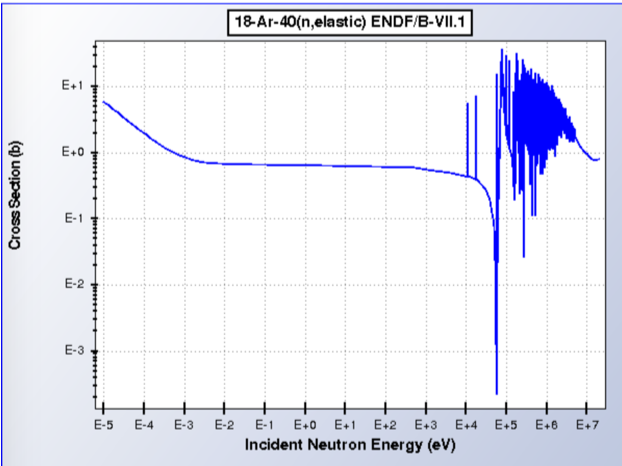
\includegraphics[width=0.4\linewidth]{Figures/Ar40xsec.png}
%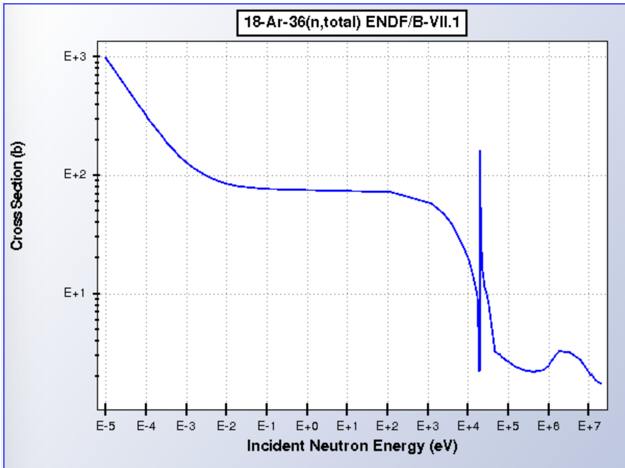
\includegraphics[width=0.4\linewidth]{Figures/Ar36xsec.png}
%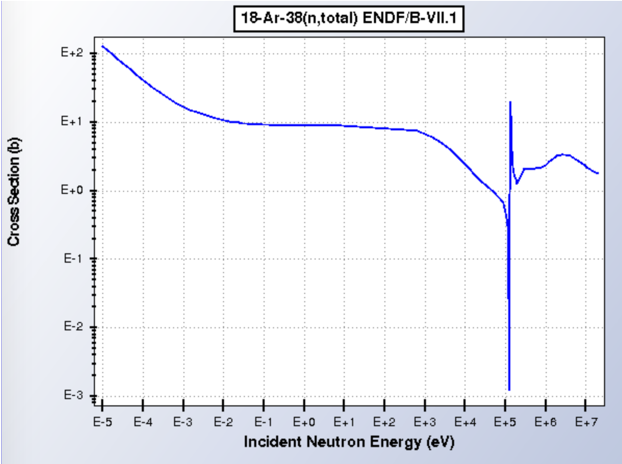
\includegraphics[width=0.4\linewidth]{Figures/Ar38xsec.png}
%\caption{Elastic scattering cross sections on 40-Ar (top left), 36-Ar (top right), and 38-Ar (bottom). From ENDF/B-VII.1~\cite{ref:ENDF}. The large anti-resonance at $57\; keV$ in 40-Ar can be clearly seen.
%{\bf NOTE: PUT IN PLOTS FOR ELASTIC}
%}
%\label{fig:Arxsec}
%\end{center}
%\end{figure}


%\begin{figure}[h]
%\begin{center}
%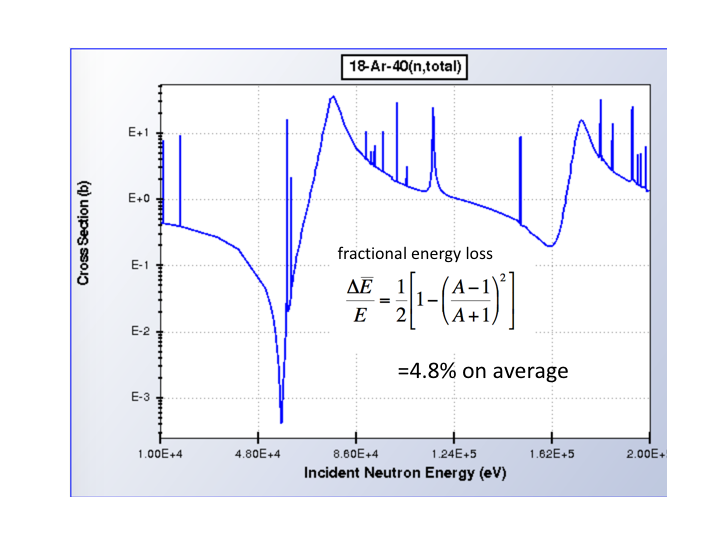
\includegraphics[width=0.75\linewidth]{Figures/Ar40Xsec2.png}
%\caption{Total scattering cross sections on 40-Ar in the range $10-200\; keV$~\cite{ref:ENDF}}
%\label{fig:Arxsec2}
%\end{center}
%\end{figure}

Liquid argon is near transparent to neutrons with an energy near or at 57~keV due to an anti-resonance in the cross-section caused by the destructive interference between two high level states of the $^{40}$Ar nucleus. The cross-section at the anti-resonance ``dip" is about 10~keV wide, and at the bottom the cross section of $1.6\times 10^{-4}\;$b implies an elastic scattering length of over $2,000\;$m. %Of course, natural 
Natural argon has three major isotopes: 36-Ar (0.3336\%), 38-Ar (0.0834\%), and 40-Ar (99.6035\%) each with a slightly different anti-resonance. The average elastic scattering length of the 57~keV neutrons in natural liquid argon is about $30\;$m.

The neutrons at the anti-resonance energy could be injected into liquid argon TPC, provided no material (e.g. hydrocarbons) blocks the path. Those that do scatter lose energy, leave the anti-resonance, quickly slow down and are captured. Each capture releases exactly the binding energy difference between $^{40}$Ar and $^{41}$Ar, about $6.1\; MeV$ in the form of $\gamma$ rays.  As will be described below, by using a {\it DD} Generator (where {\it DD} stands for "Deuterium-Deuterium"), a triggered pulse of neutrons can be generated outside the TPC, then injected via a dedicated hole in the insulation into the liquid argon, where it spreads through the 58~m volume of the detector to produce $6.1\; MeV$ energy depositions.
%Using this method, the calibration procedure would be quick (likely a few hours depending on the neutron yield of the DD generator), and there is no need to manufacture short-lived isotopes at an external facility.

The neutron capture $\gamma$ spectrum has been measured and characterized. Recently, the ACED Collaboration performed a neutron capture experiment using  the Detector  for Advanced  Neutron  Capture  Experiments  (DANCE)  at the  Los  Alamos  Neutron  Science  Center  (LANSCE). The result was published~\cite{aced} and will be used to prepare a database for the neutron capture studies.

%{\it Mention Test at LANSCE and its role?}

%%%%%%%%%%%%%%%%%%%%%%%%%%%%
\subsubsection{Design}
\label{sec:sp-calib-sys-pns-des}

The basic design concept of such a pulsed neutron source has been used successfully for Boron Neutron Capture Therapy\cite{KOIVUNORO2004853}. The design of the Pulsed Neutron Source used for energy calibration is shown in Figure~\ref{fig:PNS_Moderator}. The system will consist of four main components: a $DD$ generator, an energy moderator reducing the energy of the $DD$ neutrons down to the desired level, and the shielding materials, and a neutron monitor to confirm neutron flux and safe operation. 

\begin{figure}[tpb]
\centering
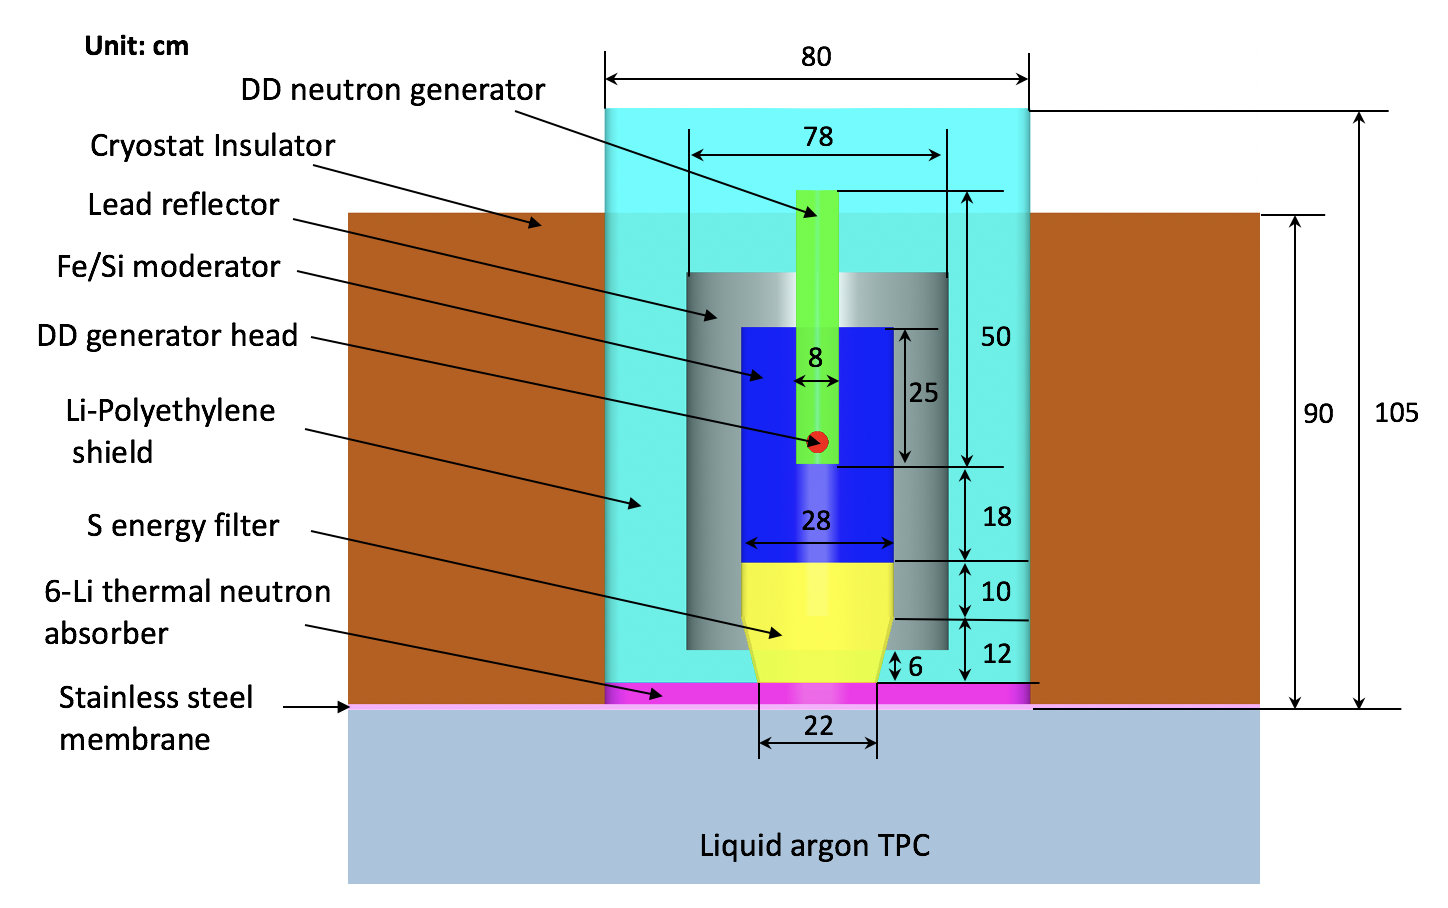
\includegraphics[width=12cm]{graphics/PNS_Moderator.png}
\caption{Conceptual design of the Pulsed Neutron Source. The whole device is placed outside the TPC volume on top of the cryostat.}
\label{fig:PNS_Moderator}
\end{figure}

{\bf DD generator source:} $DD$ generators are commercial devices that can be readily obtained from several vendors at a cost of about \$~125k each, which includes all control electronics. The pulse width is adjustable and can be delivered from about 10-1000~$\mu$s (which affects the total output). 

{\bf Moderator:}  A feasible moderator has been designed using a layered Moderator (Fe or Si)-Filter(S)-Absorber(Li) %layered 
configuration. The 2.5~MeV neutrons from the $DD$ generator are slowed down to below 1~MeV by the energy moderator. Natural iron and silicon are found to be efficient moderators for this purpose. Then an energy filter made of sulfur powder is used to further select the neutrons with desired anti-resonance energy.
The neutron anti-resonance energy in $^{32}$S is 73~keV, right above the 57~keV anti-resonance energy in $^{40}$Ar. The neutrons at this energy lose about 3.0~keV per elastic scattering length. After a few elastic scattering interactions, most of the 73~keV neutrons selected by the sulfur filter will fall into the 57~keV anti-resonance energy region in liquid argon. These materials require no cooling or special handling. Finally, a thermal absorbing volume of Lithium is placed at the entry to the argon pool in order to capture any neutrons that may have fallen below the 57~keV threshold. The reflecting volume is added around the $DD$ generator and the neutron moderator to increase downward neutron flux. 

{\bf Shielding:} The source will be encased in a shielding volume. The goal of the shield is to block both scattered neutrons and gammas which are produced in the source. Lithium-Polyethylene (7.5~$\%$) is chosen to be the material for the neutron shield because it is rich in hydrogen and lithium atoms which yield a high neutron absorption cross section. Lithium-Polyethylene is also light weight, commercially available, and relatively inexpensive. The energy spectrum entering the shield has multiple peaks between 0.5~MeV and 1.5~MeV, and one major spike at 2.2~MeV. The shield is able to effectively block the lower energy peaks but is only able to degrade the intensity of the 2.2~MeV peak. This is because 2.2~MeV gammas are a characteristic signature for neutron captures on hydrogen. A safe thickness of the lithium-polyethylene shield must be found such that it is capable of degrading the dose of 2.2~MeV gammas to safe levels. The dose of radiation from 2.2 MeV gammas was then calculated assuming a person standing 1~m away. Simulation indicates that 12~cm of Lithium-Polyethylene shield satisfies basic safety requirements. 

{\bf Neutron Monitor:} The system will need a monitoring system to confirm the source is operating as expected.  A neutron monitoring detector consisting of an Eljen EJ-420 coupled to an ADIT L51B16S 2-inch PMT will be placed just outside of the moderating material surrounding the $DD$ generator and will be read out with a CAEN waveform digitizer with neutron/$\gamma$ pulse-shape discriminating firmware. The monitoring detector will provide relative flux information to the calibration users and will ensure that the intensity of the source is constant, thereby allowing a comparison of data taking at different times.  A small collimator will be placed in front of the neutron detector, and inside the shielding material of the $DD$ source. The collimator dimensions and material specifications (likely a combination of iron, lead, and polyethylene) will be optimized from Monte Carlo simulations.

Based on the general concept, two different designs were studied with GEANT4 simulation. Figure~\ref{fig:PNS_source_design} shows a conceptual layout of the neutron injection system. %\todo{For v2, confirm updated figure; minor error in current one.}

\begin{figure}[tpb]
\centering
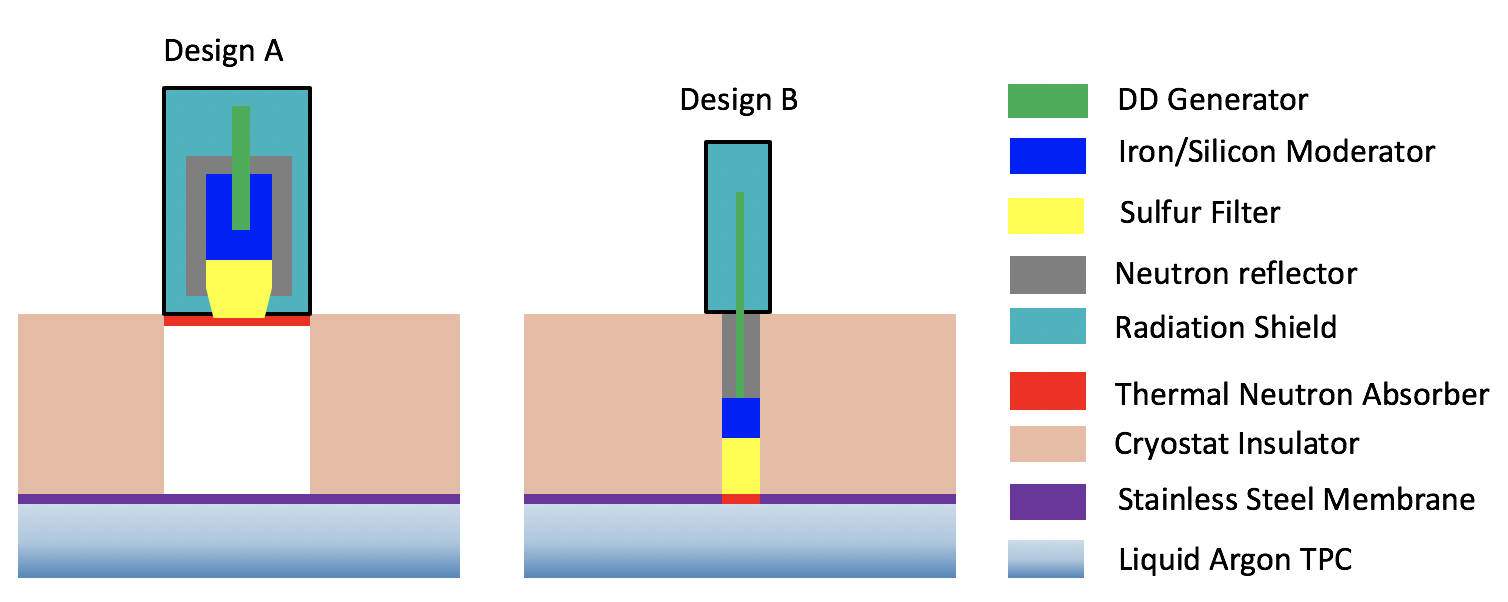
\includegraphics[width=16cm]{graphics/PNS_Two_Designs.png}
\caption{Two designs currently under development for the Pulsed Neutron Source. Design A: Large format neutron source to be deployed above/inside the human access holes or other delicate neutron injection ports; Design B: Small format neutron source to be deployed inside the calibration feedthrough ports.
%, see text for more details.
}
\label{fig:PNS_source_design}
\end{figure}

\begin{itemize}
\item Design A: Large format Moderator; \\
The neutron source is about 0.8~m wide and 1~m high. It would sit above the cryostat insulator. Beneath the neutron source, a cylinder insulator volume with a diameter of more than 50~cm has to be removed to allow the neutrons to get into the cryostat. Such an interface is provided by the human access ports near the endwalls of the detector; a picture of this is shown for \dword{protodune} in Figure~\ref{fig:humanaccessport}. The top flange is sealed, and the neutron source sits on top (Design A), providing heat insulation; The neutron source weighs about 1.6~tons and will hang on the I-beam supporting structure. This design allows a permanent deployment of the neutron source. GEANT4 simulation has shown that 0.13 ~\% of the neutrons generated by the $DD$ generator are expected to be captured inside the liquid argon TPC. It is also possible to place the neutron source inside the human access port which would allow a factor of 6 increase of the neutron flux but require a modification of the interface flange. This is currently being investigated.
% JW: I think It doesn't harm to mention that the neutron source could be placed inside the manhole. My recent simulation is based on this configuration.

%\item \fixme{KM: I do not think this is possible for quite a few reasons-- heat loss and also cost of adjusting this. Remnoving this for now.} Design B: Large format Moderator; no insulation between Moderator and cryostat membrane The design of the the neutron source itself would be same as Design A. The only difference is that the neutron source will be placed inside a hole on the cryostat insulator. The cryostat will be kept closed, but there is no vacuum insulation between the neutron moderator and the stainless steel membrane. As the neutron source is closer to the liquid argon cryostat, the neutron flux is expected to be a factor of 10 higher than that of Design A. However, the neutron source must be removed and the insulator has to be recovered after the calibration run. 
\item Design B: Small format Moderator; no insulation between Moderator liquid argon. An alternative method for delivering the neutrons is to use the existing calibration feedthroughs. In the current cryostat design, 20 calibration feedthroughs with a 20~cm inner diameter will be available on top of the cryostat. One can design the neutron source with an ultra-thin $DD$ generator that fits the size of the feedthrough. The problem is that there will be no space in the feedthrough for the shielding materials to fit in, so additional shielding will need to be placed around the feedthrough. The weight of this compact neutron source will be about 140~kg, so mounting will be simpler compared to Design A. The effective neutron flux is expected to be similar as that of Design A. 
\end{itemize}

\begin{figure}[tpb]
\centering
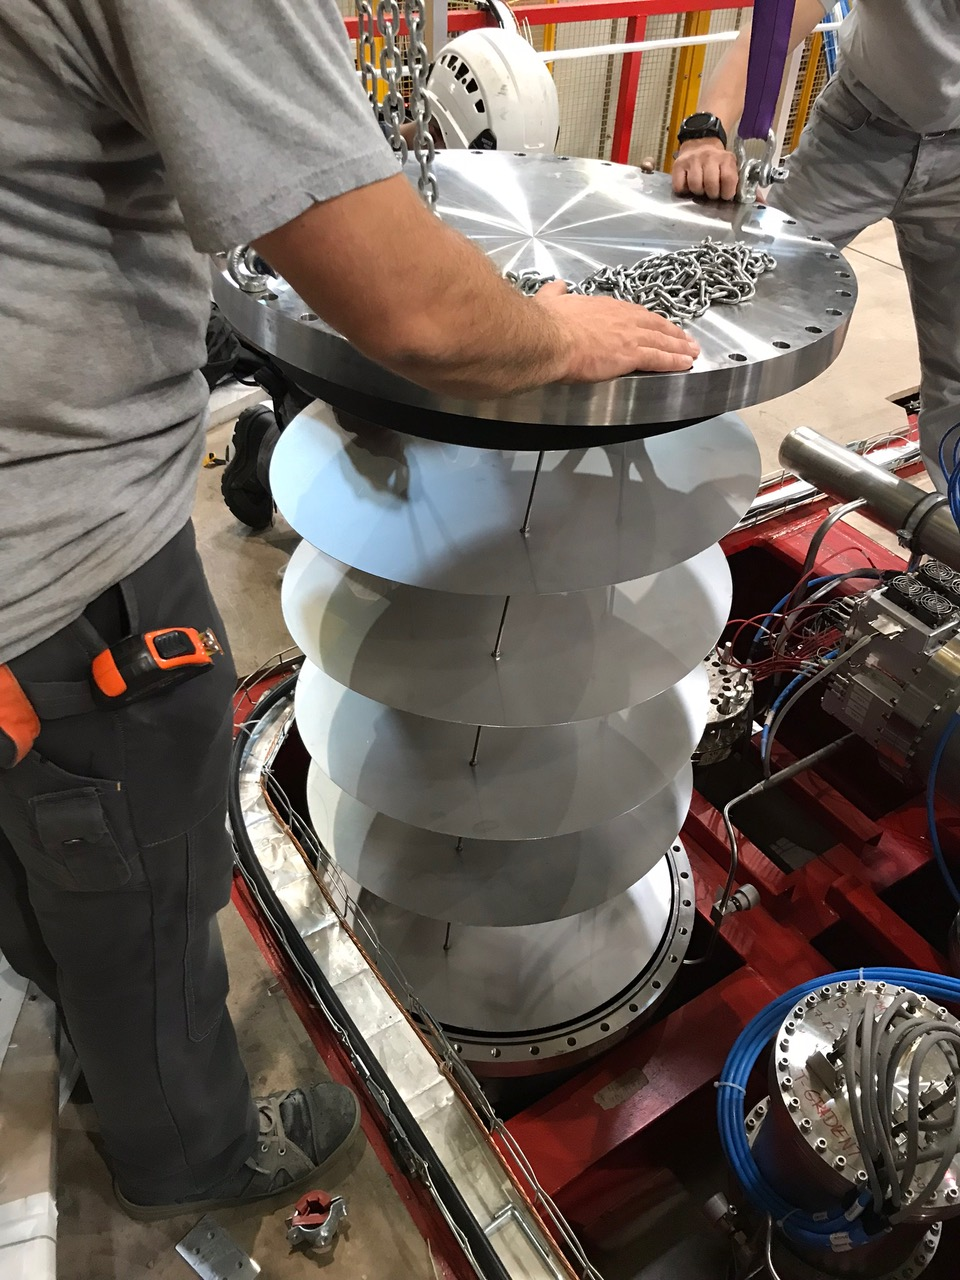
\includegraphics[width=6cm]{graphics/manhole2.jpg}
\caption{Flange for human access port on ProtoDUNE-SP and support structure (red frame).}
\label{fig:humanaccessport}
\end{figure} 

\begin{figure}[tpb]
\centering
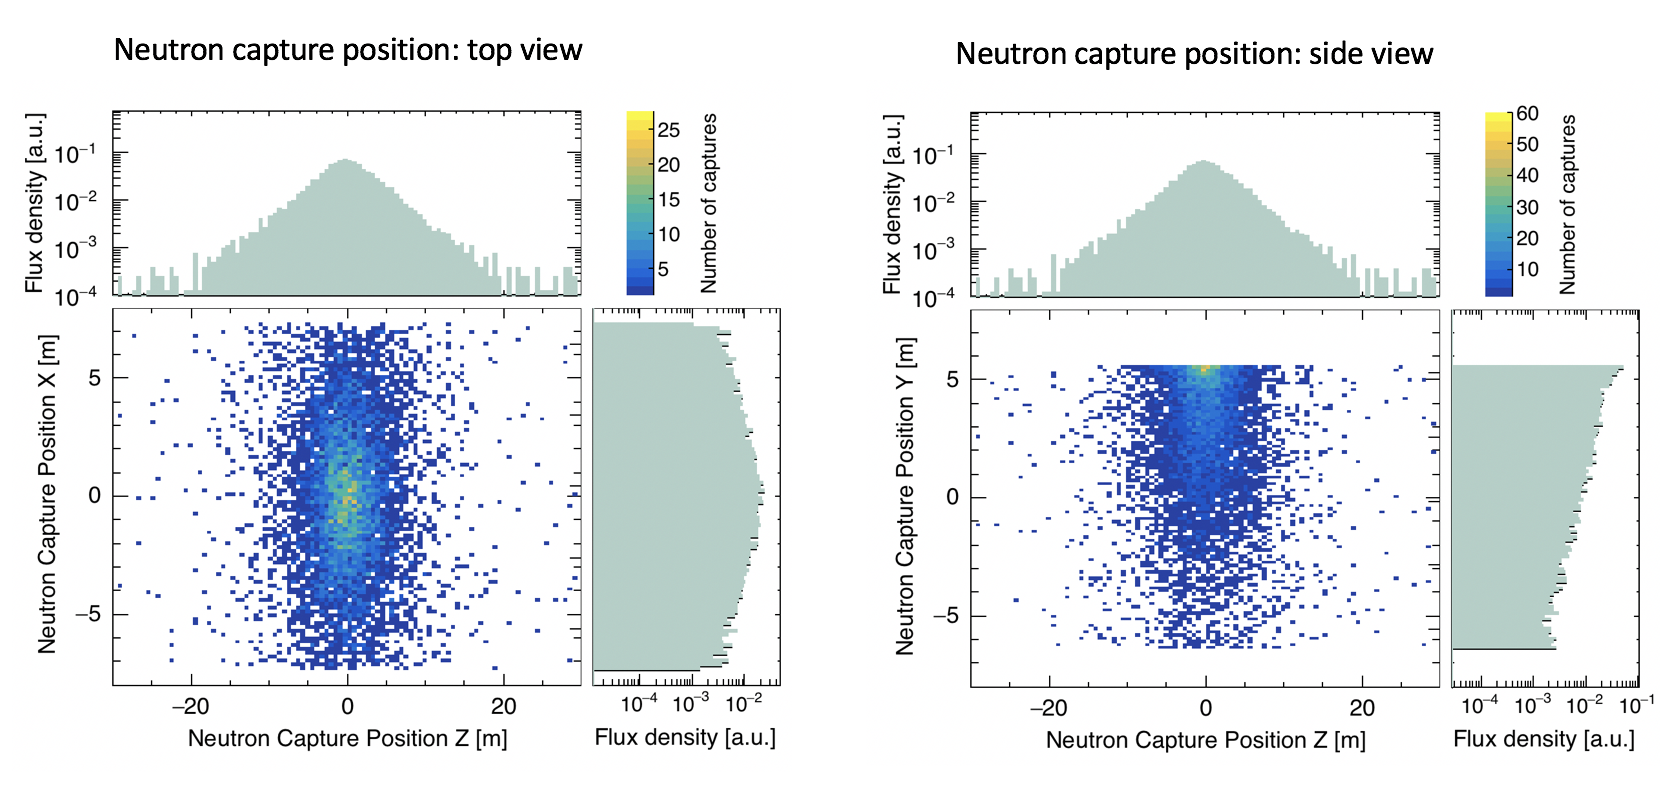
\includegraphics[width=18cm]{graphics/PNS_NcapPosition.png}
%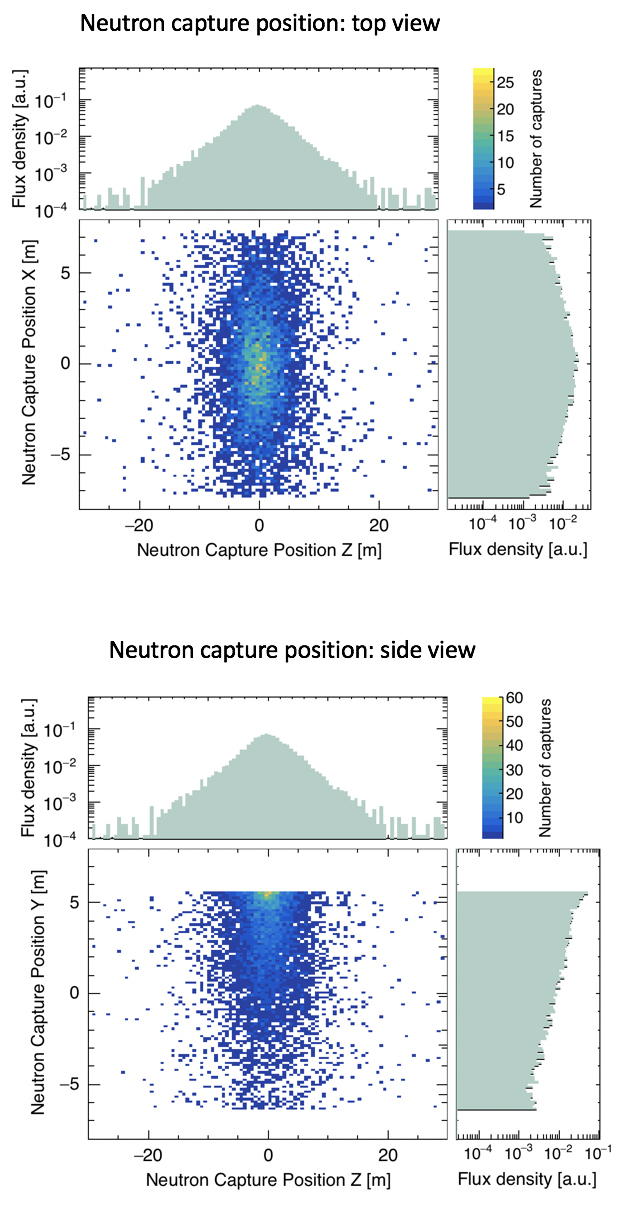
\includegraphics[width=10cm]{graphics/PNS_NcapPosition_v2.png}
\caption{Neutron capture positions inside a DUNE sized TPC. L=60~m (along Z axis, horizontally parallel to the beam direction), W=14.5~m (along X axis, horizontally perpendicular to the beam direction), H=10~m (along Y axis, vertically perpendicular to the beam direction). The neutron moderator is based on Design A, but the entire source is placed inside the injection port that is central to the cryostat. 10$^{6}$ DD generator neutrons with 2.5~MeV energy were simulated in the moderator and propagated inside the liquid argon TPC. Left: Top view of neutron capture positions. Right: Side view of neutron capture positions.} 
\label{fig:ncapposition}
\end{figure} 

The two designs were simulated in GEANT4. The position distribution of the neutron captures is shown in Fig.~\ref{fig:ncapposition}. In the simulation, the Pulsed Neutron Source is placed on top of the liquid argon cryostat with the same size as the DUNE 10~kton TPC. Initial simulation results indicate that one Pulsed Neutron Source could cover half the TPC volume, so two identical neutron sources, each central to half the cryostat top,  %\todo{SG: I assume this is with design A, right? if so, mention which design}
would illuminate the whole TPC volume of the DUNE far detector for both designs. However, this would require opening two additional neutron injection ports which are not included in the current cryostat design \footnote{Ideally,opening two identical neutron injection ports for each 10~kton TPC would make full use of the neutron source. The possibility requires further discussion with the cryostat engineers.}. Alternatively, two large format neutron sources (Design A) could be permanently deployed at the human access holes at the corners of the cryostat. One concern is that the neutrons scattered from the liquid argon volume from the human access holes may not reach the center of the TPC. This can be mitigated by using a small format neutron source (Design B) deployed on top at the center of the cryostat using the multi-purpose feedthroughs. %could be used to complement the coverage of the large format sources. 
Figure~\ref{fig:PNS_energy_design} shows the energy spectrum of the neutrons moderated and injected to the liquid argon TPC, based on Design A.
% This figure is based on Design A moderator placed inside the manhole. We can still use this figure, because the energy spectrum shape should be same. Only the flux will be a factor of 6 lower
%The neutron energy is moderated from 2.5 MeV to below 100 keV.  

\begin{figure}[tpb]
\centering
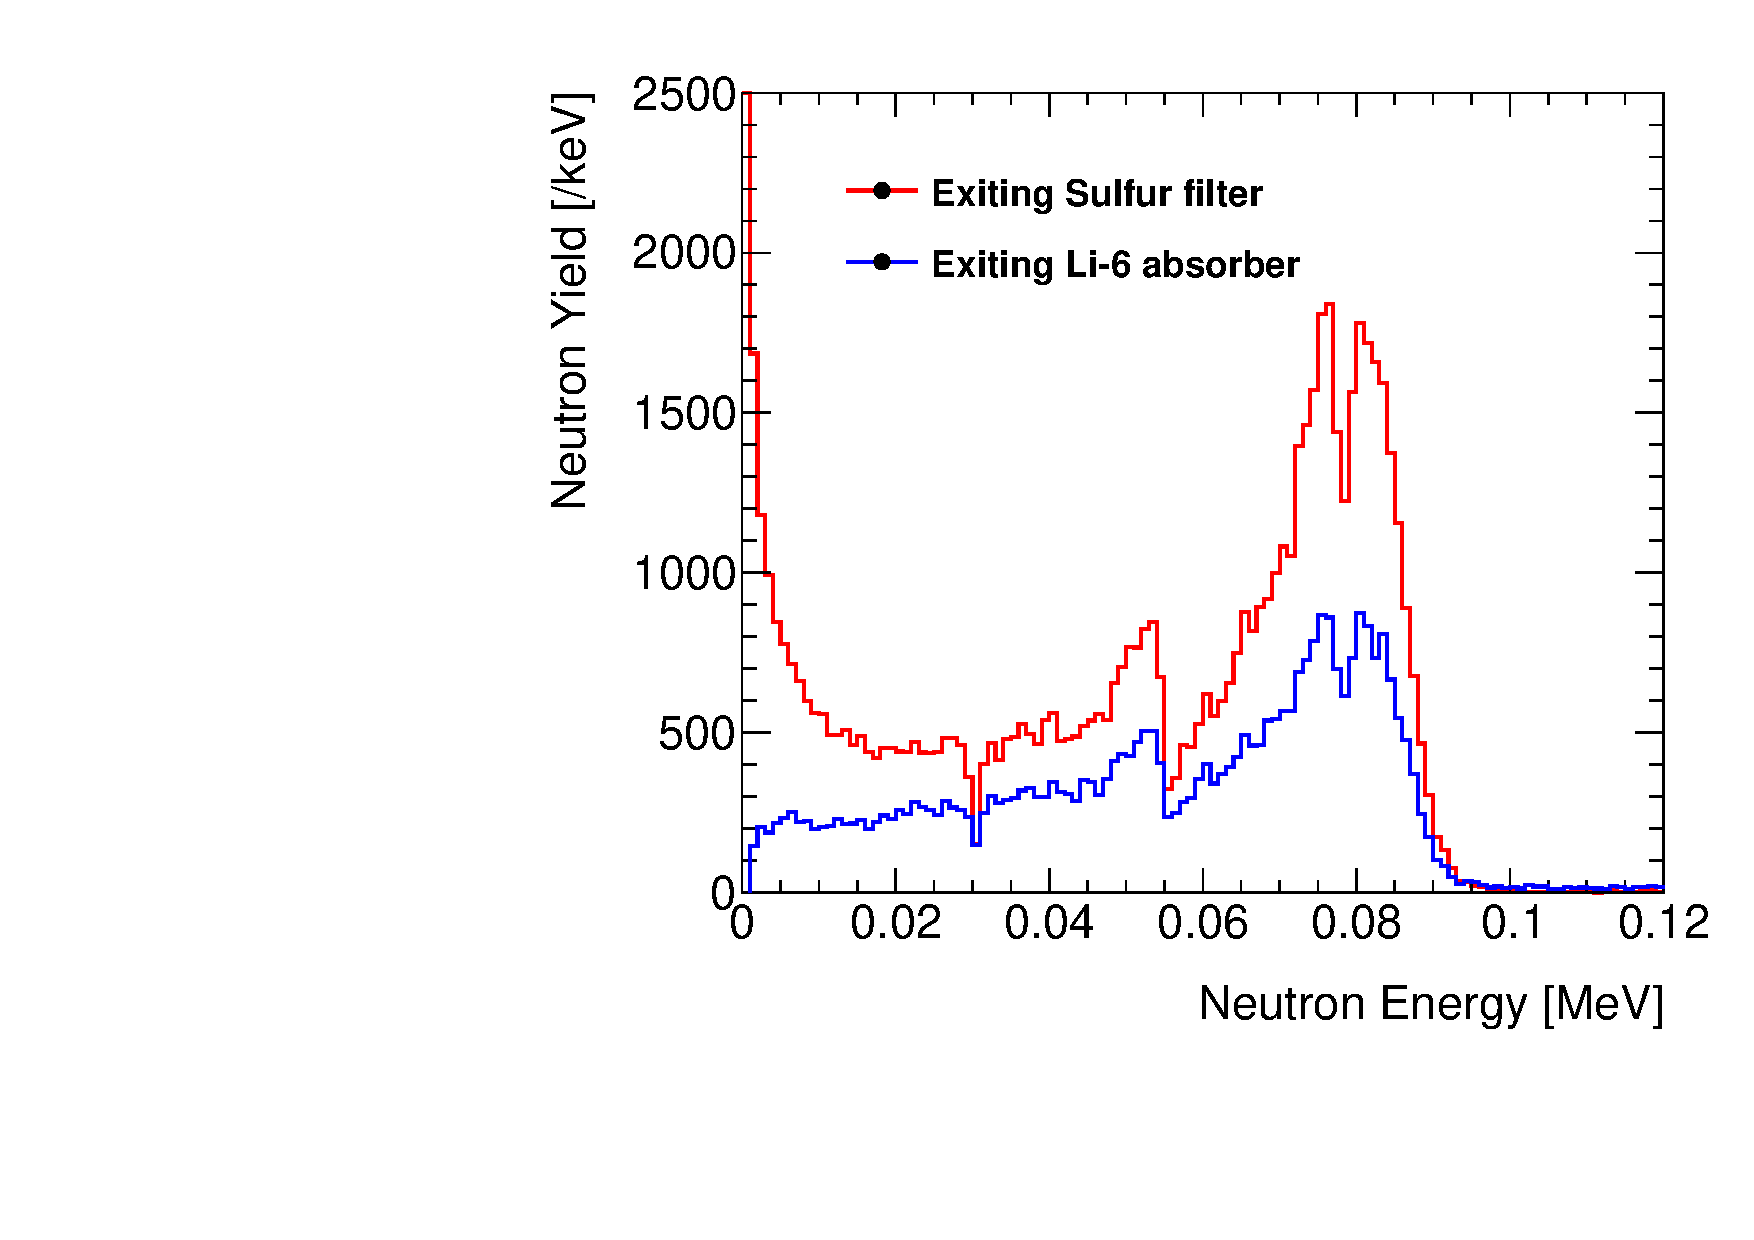
\includegraphics[width=10cm]{graphics/PNS_Energy_Moderator.pdf}
\caption{Energy of moderated neutrons produced by the Pulsed Neutron Source. Simulation is based on Design A. The total number of initial DD generator neutrons is 10$^{6}$ }
\label{fig:PNS_energy_design}
\end{figure} 

The system is expected to have a long lifetime of operation, but as the PNS system sits on top of the cryostat, with no opening to the liquid argon, it is possible to replace the system if it fails with only crane support.


%%%%%%%%%%%%%%%%%%%%%%%%%%%%
\subsubsection{Possible Measurements}
\label{sec:sp-calib-sys-pns-meas}

The 6.1~MeV $\gamma$ cascade will provide a uniform signal for neutron capture, part of the supernova signal. The source may also be used determine the relative efficiency across the detector for neutron capture, and also provide measurements of energy resolution and energy scale spatially and temporally resolved. Simulation studies are currently underway and for the second draft, we plan to include a first round of simulation results.

%\todo{Simulation studies are underway but changing rapidly. for v2 we will include a first round of studies.}







%%%%%%%%%%%%%%%%%%%%%%%%%%%%%%%%%%%%%%%%%%%%%%%%%%%%%%%

\subsection{Proposed System: Radioactive Source Calibration System}
\label{sec:sp-calib-sys-rs}

% \fixme{Call it "deployment" or "calibration" system?}
%%%%%%%%%%%%%%%%%%%%%%%%%%%%%%%

%\fixme{KM: done for now, but am not satisfied with the end of it-- Juergen did not provide measurements! SG/JM: please briefly check to make sure it is coherent? SG: done. Sent an email to Juergen with some items to be addressed.}

\subsubsection{Physics Motivation}

Radioactive source deployment provides an in-situ source of physics signals at a known location and with a known activity that can be chosen such that there is only one calibration event per drift time window. The baseline source design probes de-excitation products (gamma-rays) which are directly relevant for detection of supernova neutrinos and/or $^{8}B$ solar neutrinos. Secondary measurements from the baseline source deployment include electro-magnetic (EM) shower characterization for long-baseline $\nu_e$ CC events, electron lifetime as a function of  \dword{detmodule} vertical position, trigger efficiency study versus threshold, and help determine radiative components of the Michel electron energy spectrum from muon decays. Aside from the baseline source, other sources could be deployed with the same multi-purpose system that probe for example the impact of various radiological backgrounds or measure the neutron tagging efficiency, useful for improved calorimetry of beam neutrino interactions.

Both the radioactive source system and the pulsed neutron source system are needed to address integrated response of the detector for low energy physics. Response in Ar may change rapidly as a function of photon energy due to underlying nuclear physics mechanisms. A combination of 6 MeV (direct neutron capture response), 9 MeV (peak visible $\gamma$-energy of interest to \dword{snb}), and decay electrons (~30 MeV) is needed to map this response. In terms of complementarity, radioactive sources provide a known position, known-energy single photon events while the pulsed neutron source provides a simple, potentially, non-invasive design with multi-photon energy signature which is visible across the entire detector with a known time signature.


%%%%%%%%%%%%%%%%
\subsubsection{Design Considerations}

A composite source can be used that consists  of $^{252}$Cf, a strong neutron emitter, and $^{58}$Ni, which, via the $^{58}$Ni(n,$\gamma$)$^{59}$Ni process, converts one of the $^{252}$Cf fission neutrons, suitably moderated, to a monoenergetic \SI{9}{\MeV} photon~\cite{Rogers:1996ks}. 
The source is envisaged to be inside a cylindrical moderator with mass of about \SI{15}{kg} and a diameter of \SI{20}{\cm} such that it can be deployed via the multipurpose instrumentation ports discussed in Section~\ref{sec:calib-ports}. The activity of the radioactive source is chosen such that no more than one \SI{9}{\MeV} capture $\gamma$-event occurs during a single 
drift period. This allows one to use the arrival time of the measured light as a $t0$ and then measure the average drift time of the corresponding charge signal(s). The sources would be deployed outside the \dword{fc} within the cryostat to avoid regions with a high electric field, about \SI{30}{\cm} from the field cage. The $\gamma$-ray would need
to travel about two attenuation lengths (including the \SI{10}{\cm} radius of the source body). Such high
$\gamma$-energies are typically only achieved by thermal neutron
capture, which invokes a neutron source surrounded by a large
amount of moderator,
thus making such an externally deployed (n, $\gamma$) source \SI{20}{\cm}  to \SI{50}{\cm} % large
in diameter. 

In Ref.~\cite{Rogers:1996ks},
%\cite{Triumf:Nickelsource} 
%\todo{SG: reference needs fixing},
a $^{58}$Ni (n,$\gamma$) source, triggered by an AmBe neutron source,
was successfully built, yielding high $\gamma$-energies of \SI{9}{\MeV}. DUNE %We
proposes to use a $^{252}$Cf (or AmLi as backup) neutron source with lower
neutron energies, which requires less than half of the surrounding
moderator, and making the $^{58}$Ni (n, $\gamma$) source only
\SI{20}{\cm} or less in diameter. The multipurpose instrumentation
feedthroughs at either end of the cryostat are sufficient for
this, and have an inner diameter of \SI{25}{\cm}.  The moderator
material chosen for DUNE is Delrin which has a large enough
density to avoid flotation. Further, the end caps of the source
body are round to avoid distorting the electric field and to
eliminate the risk of the source getting stuck during deployment. 
Figure~\ref{fig:RadSource} depicts the baseline source design of a
cylindrical Delrin moderator with a diameter of \SI{20}{\cm}, a
height of \SI{40}{\cm} including half-spheres at either end with
radius of \SI{10}{\cm}, deployed at $z$=\SI{40}{\cm} leaving a gap of \SI{30}{\cm} towards the \dword{fc} and at a distance to the \dword{apa} of $x$=\SI{220}{\cm}, 
which is slightly further than mid-drift.

\begin{dunefigure}[h]{fig:RadSource}{Fish-line deployment scheme in DUNE for a radioactive source
encapsulated inside a cylindrical Delrin moderator body with a
diameter of \SI{20}{\cm}, a height of \SI{40}{\cm} including
half-spheres at either end with radius of \SI{10}{\cm}. A
$^{252}$Cf neutron source and a natural nickel target are sealed
inside at the center. The fish-line is deployed \SI{40}{\cm}
outside of the \dword{fc} and at \SI{220}{\cm} distance to the
\dword{apa} (red plane).}
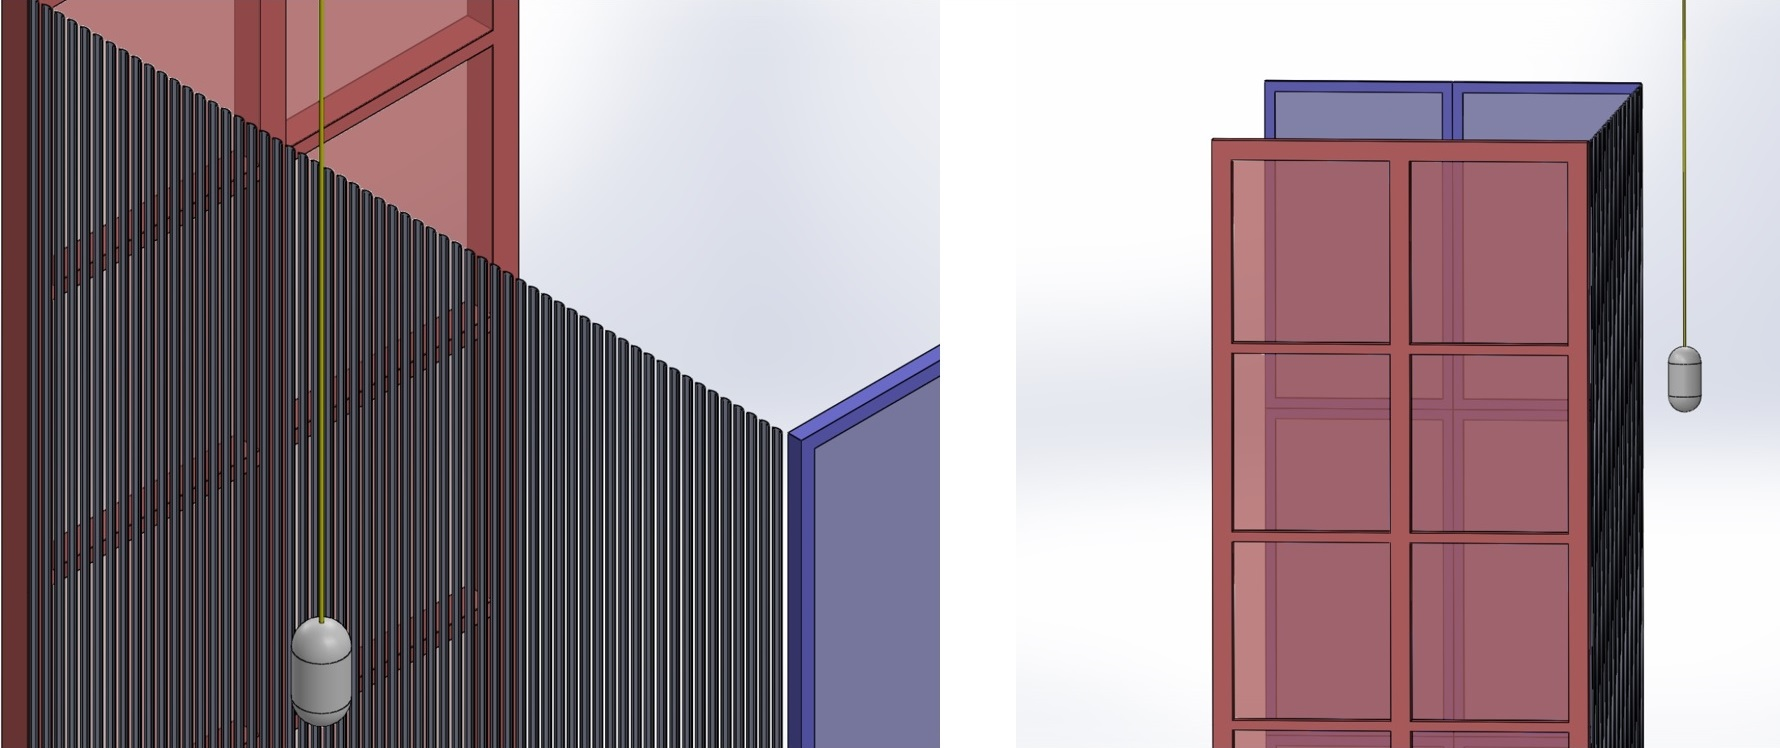
\includegraphics[width=1.0\linewidth]{RadioactiveSource_zm40cm_xp220cm.jpg}
\end{dunefigure}

% Here it is, but I don't have privileges for the bibliography

%@Misc{Triumf:Nickelsource,
%  author =   {J. Rogers, M. Andreaco, C. Moisan},
%  title =    {A $7-9$\,MeV isotropic gamma ray source for detector testing},
%  howpublished = {TRIUMF TRI-PP-96-7},
%  month =    {Apr},
%  year =     {1996},
%}

%\fixme{KM: From Juergen but I think covered by above: The activity of the radioactive source is chosen such that no more than one \SI{9}{\MeV} capture $\gamma$-ray spills into the active \dword{lartpc} region during a single \SI{2.2}{\milli\s} drift period. This allows one to use the arrival time of the measured light as $t_{0}$ and then measure the average drift time of the corresponding charge signal(s). The resulting drift velocity in turn yields the electric field strength, averaged over the variations encountered during the drifting of the charge(s). This can be repeated for each single \SI{9}{\MeV} capture $\gamma$-event that occurs during a \SI{2.2}{\milli\s} drift period and where visible $\gamma$-energy is deposited inside the active volume of the TPC. Pile-up and data read-out considerations restrict the maximally permissible event rate to less than \SI{10}{\hertz} and in turn the \SI{9}{\MeV} capture $\gamma$-rate occurring inside the radioactive source body to less than \SI{140}{\hertz}, given a spill-in efficiency into the active \dword{lar} of about \num{7}\%.}

A successfully employed multipurpose fish-line calibration
system~\cite{DCnearDetTDR} \todo{SG: Juergen to provide proper reference.} 
%\fixme{need to add reference: "The Double Chooz Near Detector Technical Design Report" 
%Double Chooz Collaboration (H. de Kerret (APC, Paris) et al.) Oct 1, 2012. EDMS ID:I-028812 ; DocDB ID: 3403-V5 Pages 198 - 223
%(Anne can't find proper ref for this)}
 for the Double Chooz
reactor neutrino experiment has become available for DUNE after
the decommissioning of Double Chooz in 2018. The system can be
easily refitted for use in DUNE. The system will be housed inside
a purge-box that is connected via a neck to a multipurpose
calibration feedthrough with a closed gate valve on top of the
cryostat. Before deployments, the purge-box will be evacuated by a
vacuum pump, then purged with argon gas, and the pressure
equalized with the gas pressure inside the detector, before the
gate-valve is opened and deployments can commence. 
%Also, if the source is in close proximity of an \dword{apa} wire frame, lower energetic radiological backgrounds become problematic as the source light and charge yield is reduced exponentially with distance. 
Near mid-drift (in each TPC module) the \SI{9}{\MeV}
$\gamma$-ray source can illuminate the full drift length from
\dword{apa} to \dword{cpa}. The sources are retrieved from the
detector after each deployment and stored outside the cryostat following approved safety protocols.

The commissioning plan for the source deployment system will include a dummy 
source deployment (within 2 months of the commissioning) followed by first real source deployment (within 3-4 months of the commissioning) and a second real source deployment (within 6 months of the commissioning). Assuming stable detector conditions, the radioactive source will be deployed every half a year. Ideally, a deployment before and after a run period are desired so at least two data points are available for calibration. This also provides a check if the state of the system
has changed before and after the physics data run.
%If stability fluctuates for any reason (e.g., electronic response changes over time) at a particular location, one would want to deploy the source at that location once a month, or more often, depending on how bad the stability is.
It is expected that it will take a few hours (e.g. 8 hours) to deploy the system at one feedthrough location and a full radioactive source calibration campaign might take %at least 
a week.

The major development plans for the radioactive source system include:
\begin{itemize}
\item Continued development of relevant simulation tools including geometry representation of the source deployment system, impact from various radiological contaminants on detector response. 
\item Studies to suppress radiological backgrounds for the calibration source
\item Simulation studies to understand data and trigger rates;
\item Build a baseline design source with Delrin moderator, $^{252}$Cf neutron source and natural nickel target, both sealed inside at the moderator's center.
\item Validate \SI{9}{\MeV} capture $\gamma$-ray yield of source by spectroscopic measurements with a germanium detector (that also has a large enough assay chamber) at South Dakota School of Mines and Technology.
\item Validate with $^{3}$He based hodoscope at South Dakota School of Mines and Technology that the flux of neutrons escaping from the moderator is not an issue (otherwise use lower energetic AmLi neutron source instead and/or more moderator material, and/or different geometric configuration of nickel target). 
\item Validate that anticipated fluid flow in \dword{lar} does not cause oscillations of the source (otherwise design vertical guide wires that will get pre-installed during detector installation and that will keep source stable in position during a deployment along the vertical axis).
\item A mechanical test of the Double Chooz fish-line deployment system with a \dword{lar} (and liquid nitrogen) mock-up column will be done in the high bay lab at South Dakota School of Mines and Technology. The ultimate test of the system will be done at ProtoDUNE. 
\item Other radioactive sources beyond the baseline design will be explored that will help understand the impact of various radiological backgrounds such as e.g. hybrid neutron sources ($^{252}$Cf and AmBe) that emulate the kinetic neutron energy spectrum of radiological neutrons and probe the neutron tagging efficiency.
\end{itemize}

A successful demonstration of the radioactive source system in ProtoDUNE-SP-II running is the main priority for this system towards making a decision on deploying this system for the \dword{fd}. A schedule with main steps towards ProtoDUNE deployment is shown in table~\ref{tab:calib-rsds-sched}.

\begin{dunetable}
[Key milestones towards commissioning the radioactive source deployment system (RSDS) in ProtoDUNE-SP-II.]
{p{0.65\textwidth}p{0.25\textwidth}}
{tab:calib-rsds-sched}
{Key milestones towards commissioning the radioactive source system in ProtoDUNE-SP-II.}  
Milestone & Date (Month YYYY)   \\ \toprowrule
Baseline RSDS design validation & January 2020 \\ \colhline 
RSDS mock-up deployment test at SDSMT & March 2020 \\ \colhline 
RSDS Design review  & May 2020 \\ \colhline
RSDS Production readiness review (PRR) & July 2020 \\ \colhline
Start of module 0 RSDS component production for ProtoDUNE-II & September 2020      \\ \colhline
End of module 0 RSDS component production for ProtoDUNE-II &  February 2021    \\ \colhline
\textbf{Start of ProtoDUNE-SP-II installation} & \textbf{March 2021} \\ \colhline
Start of RSDS installation &  April 2021    \\ \colhline
RSDS demonstration test at ProtoDUNE-SP-II  & April 2022\\ \colhline
\end{dunetable}



%%%%%%%%%%%%%%%%%%%%%%%%%%%%
\subsubsubsection{Possible Measurements}
\label{sec:sp-calib-sys-src-dep-meas}

The 9 MeV single gamma source may also be used to test the gamma aspect of the \dword{snb} signal along the full drift but only in the endwall regions of the detector. The source may also be used to determine the relative efficiency in the vertical direction for measurements of energy resolution and energy scale. Simulation studies are currently underway and for the second draft, we plan to include a first round of simulation results.

%\todo{Simulation studies are underway; for v2 we will include a first round of studies.}
 

%%%%%%%%%%%%%%%%%%%%%%%%%%%%%%%%%%%%%%%%%%%%%%%%%%%%%%%
%\section{Additional Systems Considered: External Muon Tracker}
%\label{sec:sp-calib-addl}
 
%%%%%%%%%%%%%%%%%%%%%%%%%%%%
%\subsection{External Muon Tagger}
%\fixme{you can't have just one subsection; if it's only the muon tagger, then let's put this in the section heading}
%\input{vol-sp/ch-sp-emt}

%%%%%%%%%%%%%%%%%%%%%%%%%%%%%%%%%%%%%%%%%%%%%%%%%%%%%%%
%\section{Cryostat Configuration for Calibration}
%\label{sec:sp-calib-cryocfg}


%%%%%%%%%%%%%%%%%%%%%%%%%%%%%%%%%%%%%%%%%%%%%%%%%%%%%%%  Anne changed from subsection to section
\section{DAQ Requirements}
\label{sec:sp-calib-daqreq}
%\fixme{SG: Done. JM: Done. (changed "DC" to continuously).\\
%KM/JM: Plesae check. Waiting on two things from Josh (What is "DC" used in RAS section; and which section he is referring to in the first two paragraphs?\\
%JM: Probably the DAQ Chapter of the TDR. Need to check w/ Tim/Sam if this is the right reference.}
 
%\section{DAQ Requirements}
%\label{sec:sp-calib-daqreq}

The calibration systems must interface with the DUNE data acquisition system, discussed in detail in Section~\ref{sec:daq}.
The primary interface with calibrations will be through the DUNE timing system, which is responsible for providing synchronization across all subsystems and absolute time stamps, as well as for distributing triggers. Whenever possible, it is preferred that subsystems like calibrations are triggered {\it by} the DAQ rather than providing a trigger {\it to} the DAQ. Therefore the calibration systems must be designed to accept such triggers (which will have the form of a time stamp for when a trigger should occur) and it must have a way of accepting general timing information so that it is synchronized to the rest of DUNE.

Each calibration system will nevertheless be handled slightly differently, and each will have a different way for the DAQ to handle its data.  The calibration systems could easily dominate the entire data volume for DUNE, and thus exceptions to the standard triggering and readout discussed in Section~\ref{sec:daq} are needed. We discuss below these details and the associated differences.
           
\begin{dunetable}
[Calibration DAQ summary]
{p{0.2\textwidth}p{0.15\textwidth}p{0.5\textwidth}}
{tab:calib-daq}
{Estimated DAQ rates per year per 10~kton for various calibration systems.}   
System & Data Volume (TB/year) & Assumptions  \\ \toprowrule
Ionization Laser System & 185 & 800k laser pulses, 10x10x10 cm voxel sizes, a 100~$\mu$s zero suppression window (lossy readout), and 2 times/year  \\ \colhline
Neutron Source System & 84 & 10$^{6}$~neutrons/pulse, 1000 neutron captures/m$^{3}$, 1300 observed neutron captures per pulse, 6~times/year  \\ \colhline
Proposed Radioactive Source System & 200 & Source rate < 10~Hz; single fragment readout,  lossless readout; 4 times/year   \\ \colhline

\end{dunetable}           
           
\subsubsection{Laser System}

%The proposed laser source is the only practical way to unambiguously measure the electric field vectors within the detector. 
The \efield vector from ionization laser calibration is determined by looking at the deflection of crossing laser tracks within detector voxels. The voxels are currently estimated at the size of $10\times10\times10~{\rm cm}^3$. Because any given laser track
illuminates many such voxels, one laser pulse can be used for multiple
measurements---essentially the number that matters is the area of each voxel.
The number of total laser ``events'' are estimated to be 800,000---about half the rate of cosmic rays, and thus nominally a substantial total data volume.

Fortunately, unlike every other event type in the detector, the laser track has both a reasonably well known position and time; thus tight zero-suppression can be applied for both collection and induction plane wires. %Brett Viren suggests that 
A 100~$\mu$s zero suppression window is estimated to be wide enough to
avoid windowing problems in the induction plane wire deconvolution process, and we
therefore assume such a window for the laser pulses. Note that the zero
suppression happens {\it after} the trigger, not at the front-end or in the DAQ
readout; thus the rate that the laser can be run will have to take into account
the bandwidth through the Event Builder (where the zero-suppression would
occur). From the standpoint of data volume, however, the total assuming the
100~$\mu$s zero-suppression window is:
\begin{equation}
800,000/{\rm scan/10~kton} \times 100\mu{\rm s} \times 1.5{\rm Bytes/sample}\times 2~{\rm MHz}\times 384000~{\rm channels}   = 92~{\rm TB/scan/10~kton}   
\end{equation}

If such a calibration scan were done twice/year, then the total annual data volume for the laser is 184~TB/year/10~kton.

\subsubsection{Pulsed Neutron Source}
%\todo{SG: JW to update this text and the number in the DAQ table 1.3.}
%There are two radioactive sources suggested to provide low-energy calibration data for DUNE: a neutron generator source, and a $\gamma$ source. 

The pulsed neutron source system creates a burst of neutrons which
%, because of the interesting neutron cross section of argon, 
get captured throughout a large fraction of the total cryostat volume. From a triggering and data volume
standpoint, this is very convenient: the existing scheme of taking 5.4~ms of data for each trigger means all of these neutrons will be collected in a single DUNE event. Thus the data volume is simply 6.22~GB times the total number of such pulses, but these are likely to be few: a single burst can produce thousands of neutrons whose $t_0$ is known up to the neutron capture time of 200~$\mu$s or so.


Typically, a commercial $DD$ neutron generator produces 10$^{5}$ - 10$^{8}$ neutrons/pulse, depending on the adjustable pulse width. The current assumption for neutron yield from the $DD$ generator is 10$^{6}$ neutrons per pulse\footnote{Ideal assumption based on $DD$ generators that produce highest neutron yield with a pulse width less than 100~$\mu$s. Such type of $DD$ generators are being developed in labs; commercial devices may require further development to reach this level of performance.}. With the current deployment designs in figure~\ref{fig:PNS_source_design}, about 1300 neutron captures per $DD$ generator pulse are expected to be observed inside a 10~kt module. As the suggested number for localized energy calibration is 1000 neutron captures per m$^{3}$, a total number of 4600 pulses would be needed for the calibration of a 10~kt module. Assuming there will be two identical Pulsed Neutron Sources operating in synchronization mode, 2300 pulses are needed for each calibration run. Therefore, the total data volume per run would be
\begin{equation}
2300~Pulses \times 1.5~{\rm Bytes}\times
2~{\rm MHz}\times 5.4~{\rm ms}\times384000~{\rm channels} = 14~{\rm TB/run}.
\end{equation}
Running the Pulsed Neutron Source calibration system every two months would result in a total data volume of 84~TB per 10~kton per year and running 12 times/year would result in 168~TB/year per 10~kton. 

\subsubsection{Proposed Radioactive Source System}

The proposed $\gamma$ source is somewhat more complicated to handle in the DAQ, depending on its rate. An initial proposal suggests 8 hour runs at four feedthroughs, and because only a single APA is being illuminated typically, the Module Level trigger could reduce the total data rate by issuing trigger
commands only to the readout of the currently active APA. Nevertheless, if the rate of such a source is anywhere close to one per 5.4~ms, the detector would be running 
continuously 
%in ``DC'' 
in the current scheme. Therefore we assume that the
interaction rate in the detector is 10~Hz or less.  With this rate, and with localization of events to one APA, the total data volume would be
\begin{equation}
8~{\rm hours} \times 4~{\rm FTs} \times 10~Hz \times 1.5~{\rm Bytes}\times
2~{\rm MHz}\times 5.4~{\rm ms}\times2560~{\rm channels} = 50~{\rm TB/scan}.
\end{equation}
Running this calibration 4 times/year would yield 200~TB of data in 10~kton per year.





\begin{comment}
%SG: This is not under the scope of this chapter. Needs to be moved to physics. 
\subsubsection{Intrinsic Radioactivity}

        Mike Mooney has suggested using the intrinsic $^{39}$Ar as a
calibration source. This has many advantages over either of the radioactive
source calibrations, in particular the known level of $^{39}$Ar, its uniform
distribution in the detector, and the fact that it is always there and
therefore integrates correctly over the detector livetime. The difficulty is
that because any individual $^{39}$Ar event's $x$ position is not known
(because there is no $t_0$, the distribution of these events must be used to
make measurements, thus requiring fairly high statistics.

        Mooney's proposal is that roughly 250,000 $^{39}$Ar can provide a 1\%
measurement of electron lifetime. (Note that 1\% is a reaonable goal;
if the lifetime and maximum drift time are the same, this results
in a 2\% uncertainty on energy scale which would begin to compromise DUNE's
physics program). This number of events is easily obtained with the existing
random triggers as well as every other trigger source excluding laser pulses
and front-end calibrations.

        Like all other parameters that must be calibrated, however, what is not
clear is what the spatial and temporal variations will be in the detector.
Other LAr TPCs have performed lifetime calibrations daily (using cosmic rays
primarily), and a pixelization of 1~m$^2$ is not unreasonable, leading to a
need for 250,000 events for every m$^2$ in the detector each day, or about a
1~Hz trigger rate.

        In the existing scheme, this would be overwhelmingly the dominant
source of data. Thus either the pixelization would need to be reduced (say, to
each of the TPC volumes) or a zero-suppression scheme would have to be used.
Such a zero-suppression scheme would happen post-trigger---for example, running
random triggers at 1~Hz and based upon that trigger type, zero suppressing
signals. In the current scheme, this would happen in the Event Builder but at
1~Hz the data rate would be too high. To do zero suppression upstream---say in
the APA-level readout---based on the trigger type will likely require more
hardware resources.
\end{comment}

%\subsection{External Muon Tracker}

%        An External Muon Tracker (EMT) has also been proposed, likely as a scintillator-bar telescope at the front face of the detector. The EMT would be intended to trigger on rock muons and provide a known entry position and direction for these. It is thus the only way to test reconstruction in the DUNE FD for a sample of events in the same energy regime as the beam events.

%        Because the EMT is measuring events that will already be triggered by the TPC, the additional data volume comes only from the scintillator counters themselves. Because the only information needed for these events is the time of a hit in each counter, and because only four counters are likely to be hit by each muon (two planes of $x$ and $y$), the additional data rate from the EMT is very small.  If we limit ourselves to just the rock muons and assume that four counters are hit resulting in 4 12-bit words/counter (one charge and one time each, plus the counter ID and a local timestamp, then we get a yearly total data volume of
%\begin{equation}
%735{\rm year/10 ktonne} \times 24~{\rm B/event} = 17.6~{\rm kB/year}   
%\end{equation}

%%%%%%%%%%%%%%%%%%%%%%%%%%%%%%%%%%%%%%%%%%%%%%%%%%%%%%% Anne changed from subsection to section
\section{Validation of Calibration Hardware Systems}
\label{sec:sp-calib-val}


%%%%%%%%%%%%%%%%%%%%%%%%%%%%
%\subsection{Validation of Calibration Hardware Systems}
%\label{sec:sp-calib-val}
%\fixme{Validation section. JM: Done. SG/KM: please check.}

All the designs presented above have aspects that warrant a validation in a situation as close as possible to the final one to be deployed in DUNE FD. Tests in member institute laboratories needed to converge on a baseline design are described in the earlier sections. Here, we describe the validation of a complete baseline design.

Even if there are laser calibration systems in operation in other \dword{lar} TPC experiments (e.g. MicroBooNE, future SBND runs), the stringent requirements of such a system in terms of mechanical and optical precision, long-term reliability, track length, impact on \efield in case of an alternative design, and DAQ interface all lead to corresponding goals of a test installation and operation in dword{pdsp}, that could be accomplished in the post-LS2 run. As can be seen in Fig.~\ref{fig:pDmap}, there are currently ports of the same size as DUNE-FD that could possibly be used for these tests. If a pair of ports are used, then one could even have crossing tracks within a single drift volume. 

The goal of this would be to test all aspects of the system design, installation, alignment, operation, interfaces with DAQ, analysis, etc. In \dword{pdsp}, due to its location at surface, it should be possible to obtain a measurement of the \efield map with cosmics, and compare it with the one from the laser system, in order to improve the analysis methods or identify weak points in the design. An important design parameter is the length of a laser track. Our design assumes that 20 m is possible, but microBoone has demonstrated up to 10 m, but it could be larger, and also depend on laser intensity. Measurements are limited by the size of the detector, but a way to gain information on possible higher lengths would be to make a scan with low laser intensities, such that and end of the track would visible and register how the maximum obtained track length scales with intensity. An extrapolation to the DUNE \dword{fd} laser intensity would tell us what the maximum length would be there. Such a measurement could also be done at 
MicroBOONE or SBND.

\begin{figure}[tbp]
\centering
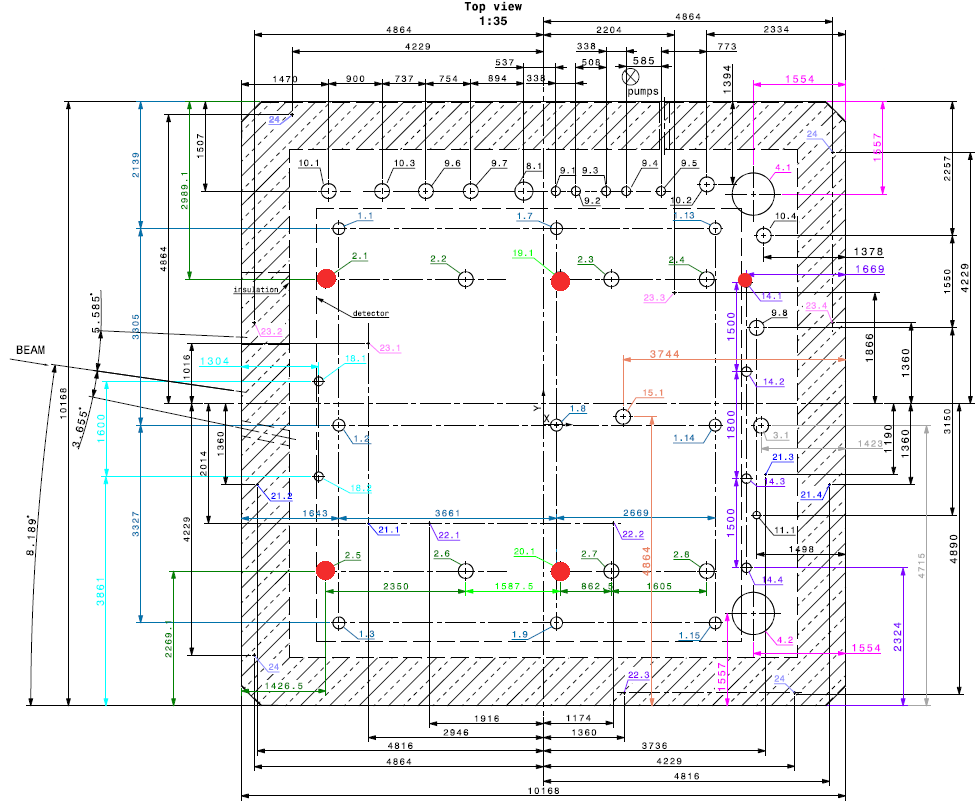
\includegraphics[height=4.0in]{graphics/protoDUNESP_topView_marked.png}
\caption{Top view of the dword{pdsp}
cryostat showing various penetrations. Ports marked in red are present free and they could be used for tests of the calibration systems. The four largest ones have the same diameter (250 mm) of the calibration ports of DUNE \dword{fd}, and are located over the TPC. The two larger ports at the right-hand side corners of the cryostat are the human access ports (or manholes).}
\label{fig:pDmap}
\end{figure}

The pulsed neutron source is a new idea that has never been used in other experiments, so a \dword{pdsp} test is especially important. The corner human access ports similar to DUNE FD could be used for this deployment.
%The post-beam run being proposed for ProtoDUNE-SP offers the opportunity to test the full system (DD Generator, Moderator, Transport Model, Data Analysis) in a definitive way before investing in the full PNS calibration for DUNE. The PNS group proposes to make such a run as soon as resources can be identified (independent of the other measurements above), starting with a commitment of engineering resources at CERN required to complete the necessary radiation safety shield design, and the mechanical design necessary to support the DD Generator and Moderator. The system used for ProtoDUNE-SP could also be used for ProtoDUNE-DP, and later installed in the DUNE detector. 

With respect to the radioactive source system, the cosmic induced background rate is too high at surface to detect the response to the DUNE gamma source; a higher intensity source can be considered to be deployed to test the detector response and analysis method. However, tests of functionality,  reliability, and safety of the mechanical deployment system are needed to demonstrate the source can be deployed and retrieved with no issues.

In addition to dedicated hardware validation runs at \dword{pdsp} running, other liquid argon experiments are providing ample opportunities for development and validation of calibration tools and techniques, especially those that are relevant for the hardware being deployed. For example, the MicroBooNE experiment is currently leading the development of analysis methods using laser data to extract an \efield map. Additionally, energy calibration techniques and related software tools are being developed at various experiments (MicroBooNE, ICARUS, LArIAT, ProtoDUNE) that involve estimating and propagating uncertainties like \efield distortions, recombination etc. into physics signals. Other calibration related developments include DAQ and calibration database design, all of which are being honed at SBN and ProtoDUNE.
 
%%%%%%%%%%%%%%%%%%%%%%%%%%%%
%\subsubsection{Validation in Other Experiments}
%\label{sec:sp-calib-val-other}

%\cleardoublepage

%%%%%%%%%%%%%%%%%%%%%%%%%%%%%%%%%%%%%%%%%%%%%%%%%%%%%%%
\section{Organization and Management}
\label{sec:sp-calib-org}


The Calibration Consortium was formed in November 2018 as a joint single and dual phase consortium, with a Consortium Leader and a Technical Leader. The organization of the consortium is shown in Figure~\ref{fig:orgchart}. The calibration consortium board currently comprises institutional representatives from 11 institutes as shown in Table~\ref{tab:gen-calib-org}. The consortium leader is the spokesperson for the consortium and responsible for the overall scientific program and management of the group. The technical leader of the consortium is responsible for managing the project for the group. 

The consortium's initial mandate is the design and prototyping of a laser calibration system, a neutron generator, and a possible radioactive source system and therefore the Consortium is organized in three working groups, each dedicated to each of these systems. Each group has a designated working group leader.
The \dword{tdr} editors are responsible for the overall editing and delivery of the \dword{tdr} document.

\begin{figure}[tbp]
\centering
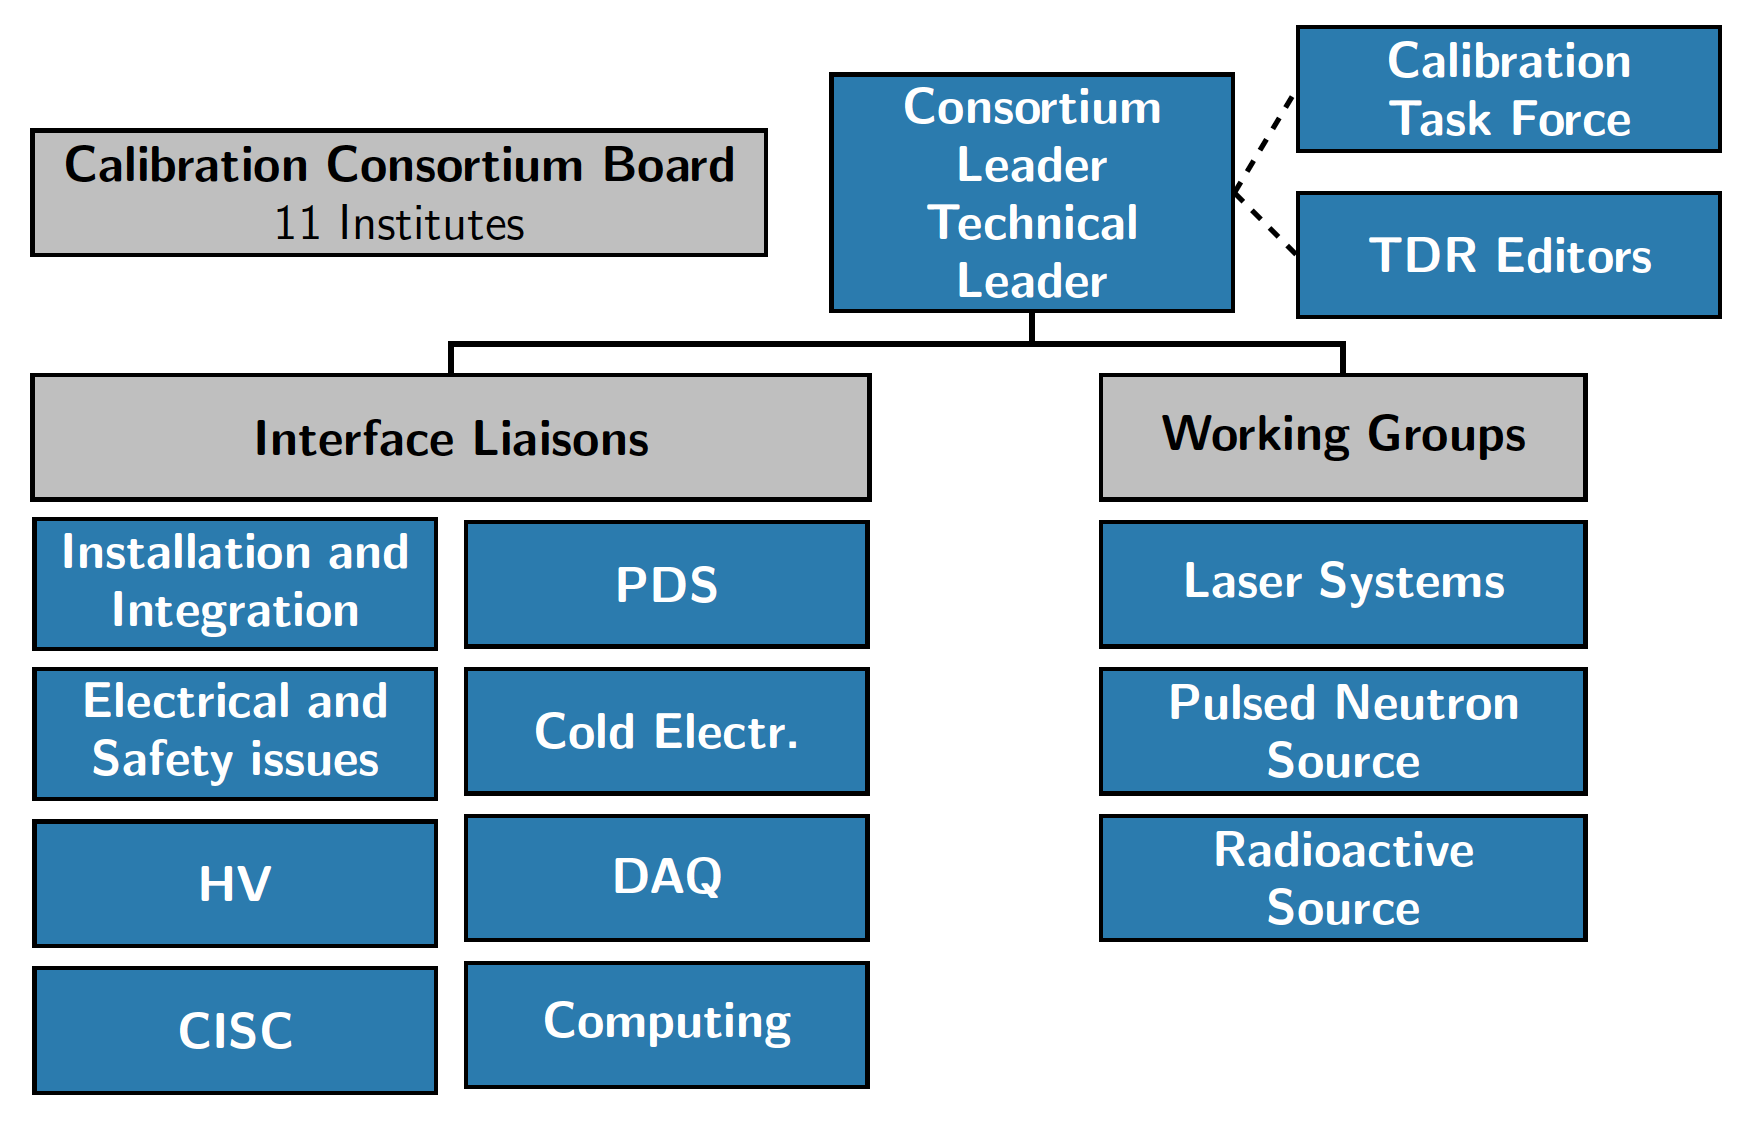
\includegraphics[height=3.0in]{graphics/orgchart.png}
\caption{Organizational chart for the Calibration Consortium.}
\label{fig:orgchart}
\end{figure}

\begin{dunetable}
[Calibration Consortium Institutions]
{lc}
{tab:gen-calib-org}
{Current Calibration Consortium Board institutional members and countries}
Member Institute     &  Country       \\
LIP & Portugal \\ \colhline
University of Bern (Bern) & Switzerland \\ \colhline
University of Tennessee, Knoxville (UTK) & USA \\ \colhline
Michigan State University (MSU) & USA \\ \colhline
Colorado State University (CSU) & USA \\ \colhline
University of Iowa & USA \\ \colhline
University of Hawaii (Hawaii) & USA \\ \colhline
University of Pittsburgh (Pitt) & USA \\ \colhline
Boston University (BU) & USA \\ \colhline
University of California, Davis (UC Davis)& USA \\ \colhline
South Dakota School of Mines and Technology (SDSMT) & USA \\ \colhline
\end{dunetable}

In addition, as shown in Fig.~\ref{fig:orgchart}, there are several liaison roles that are currently being established 
%\todo{These are being established after we have had initial interfaces and critical issues clarified} 
to facilitate the connection with other groups and activities:
\begin{itemize}
    \item Detector Integration and Installation
    \item Electrical and Safety Issues
    \item DAQ
    \item Computing
    \item Cryogenic Instrumentation and Slow Controls
    \item Cold Electronics
    \item High Voltage
    \item Photon Detection System
\end{itemize}

%\fixme{KM adjusted above from "planned" to state will exist by Summer 2019}

Currently, members from new institutes are added to the consortium based on consensus from the consortium board members following an expression of interest petition from the new institute.

%There are 11 institutes in the Consortium and, as the activities progress from design to prototyping, formalization of a Consortium Board is also planned.

%%%%%%%%%%%%%%%%%%%%%%%%%%%%%%%%%%%%%%%%%%%%%%%%%%%%%%%

\section{Interfaces}
\label{sec:sp-calib-intfc}



Interfaces between calibration and other consortia have been identified and appropriate documents are being developed that will be maintained in DUNE DocDB
%\todo{documents being prepared now}
. A brief summary is provided in this section. Table~\ref{tab:fdgen-calib-interfaces} lists the 
interfaces and corresponding DocDB documents where available. 
The main interfacing systems are \dword{hv}, \dword{pds} and \dword{daq} and the main issues that need to be considered are listed below.

\begin{description}
    \item[HV] Evaluate the effect of the calibration hardware, especially the laser system periscopes, on the \efield, even in case of no penetration of the \dword{fc}; \dword{fc} penetrations for laser. Evaluate the effect of the incident laser beam on the CPA material (kapton); Integrate the hardware of the %alternative 
    photoelectron laser system (targets) and the laser positioning system (diodes) within the \dword{hv} system components. Ensure the radioactive source deployment is in a safe field region and cannot do mechanical harm to the field cage.
    \item[PDS] Evaluate long term effects of laser light, even if just diffuse or reflected, on the scintillating components (TPB plates) of the PDS; Establish a laser run plan to avoid direct hits; Evaluate the impact of laser light on alternative PDS ideas, such as having reflectors on the CPAs. Validate light response model and triggering for low energy signals.
    \item[DAQ] Evaluate DAQ constraints on the total volume of calibration data that can be acquired, and develop strategies to maximize the data taking efficiency with data reduction methods; Study how to implement a way for the calibration systems to receive trigger signals from DAQ, in order to maximize supernova live time.
    %\item[Computing] Evaluate any additional semi-offline processing needs. Coordinate needs for calibration databases. 
\end{description}

Integrating and installing calibration devices will interfere with other devices and must be coordinated with the appropriate consortia as needed. Similarly, calibration will have significant interfaces at multiple levels with facilities to coordinate resources for assembly, integration, installation and commissioning (e.g. networking, cabling, safety etc.). Rack space distribution and interaction between calibration and other modules from other consortia will be managed by \dword{tc} in consultation with those consortia.

\begin{dunetable}
[Calibration system interface links]
{p{0.14\textwidth}p{0.40\textwidth}p{0.14\textwidth}}
{tab:fdgen-calib-interfaces}
{Calibration Consortium interface links}   
\small
Interfacing System & Description & Reference \\ \toprowrule
\dword{hv}	&
effect of calibration hardware (laser and radioactive source) on \efield and field cage; laser light effect on \dword{cpa} materials, field cage penetrations; attachment of positioning targets to HV supports 
& --- 
\\ \colhline
\dword{pds}	& 
effect of laser light on \dword{pds}, reflectors on the \dword{cpa}s (if any); validation of light response and triggering for low energy signals 
& ---  
\\ \colhline
\dword{daq}	& 
DAQ constraint on total volume of the calibration data; receiving triggers from DAQ
& ---  
\\ \colhline
\dword{cisc} &
multi-functional \dword{cisc}/calibration ports; space sharing around ports; fluid flow validation; slow controls and monitoring for calibration quantities 
& \citedocdb{7072} 
\\ \colhline
TPC Electronics	         &  
Noise, electronics calibration
& ---  
\\ \colhline
\dword{apa}	&
\dword{apa} alignment studies using laser and impact on calibrations
& --- 
\\ \colhline
Physics	&
tools to study impact of calibrations on physics
& --- 
\\ \colhline
Software \& Computing	  &
Calibration database design and maintenance
& ---
\\ \colhline
TC Facility              &   
Significant interfaces at multiple levels   
& ---   \\ \colhline
TC Installation     	  &     
Significant interfaces at multiple levels
& ---   \\ \colhline
%TC Integration Facility    &    
%Significant interfaces at multiple levels
%& ---   \\ 
\end{dunetable}

%\fixme{sample from HV - use as template; see Sec 3.5 of guidance doc}

%\begin{dunetable}
%[High Voltage System Interface Links]
%{p{0.4\textwidth}p{0.2\textwidth}}
%{tab:HVinterfaces}
%{High Voltage System Interface Links }   
%Interfacing System & Linked Reference \\ \toprowrule
%CISC & \href{http://docs.dunescience.org/cgi-bin/ShowDocument?docid=6787&version=1}{DocDB 6787} \cite{bib:docdb6787} \\ \colhline
%DP CRP & \cite{bib:docdb6754} \\ \colhline
%... & \cite{} \\ \colhline
%(last item)& \cite{} \\
%\end{dunetable}

%%%%%%%%%%%%%%%%%%%%%%%%%%%%%%%%%%%%%%%%%%%%%%%%%%%%%%%
\section{Cost and Labor}
\label{sec:sp-calib-cost}


%\fixme{KM/JM: Done; SG check?}
%KM: I am OK with this, let's see what the editors hate. \fixme{SG: done checking; 1. photoelectron laser missing from the table. Added it. 2. Updated the text to clearly state what the cost estimates include; 3. added some description for labor and a table with placeholders for actual labor hours. 4. The way it is currently split in the cost table, using the same rows will be tricky for labor hours. E.g. for the laser itself, no significant labor is associated. So, for the labor table, although it inconsistent with the cost table, I listed each of our devices as one entity. check if you are okay with this. Alternatively, we can lump everything into one system for the cost table as well so both tables are consistent which is what is expected from main editors. 5. I added a new category for labor, "physics & simulation" as those hours will also need to accounted for. }

\begin{dunetable}
[Calibration System Cost Summary]
{p{0.15\textwidth}p{0.1\textwidth}p{0.15\textwidth}p{0.4\textwidth}}
{tab:calib-cost}
{Cost estimates for different calibration subsystems.  All cost estimates include packing and shipping costs.}   
System & Quantity & Cost (under development) (k\$ US) & Description \\ \toprowrule
laser & 17 & - & high intensity laser source for laser system  \\ \colhline
laser optics module & 20 & -&  insulator ingress into detector and flange interface, mirrors, power, cables for laser system, and positioning system \\ \colhline
Photoelectron system & 4000 & - & includes targets to be mounted, both dots and strips, along with optical fibers to illuminate the photoelectric targets on two cathode planes, on both sides of each  cathode plane \\ \colhline 
DD generator device  & 2 &- & neutron source for pulsed neutron source system. \\ \colhline
Other PNS components  & 2 & - & includes moderator, surrounding shielding and neutron monitor \\ \colhline
%laser device & 17 & \num{50.0} & Laser system \\ \colhline
%feedthrough interface & 20 & \num{100.0} & Laser system; includes insulator ingress into detector and flange interface, mirrors \\ \colhline
%DD generator device  & 2 & \num{102.5} & Pulsed Neutron Source \\ \colhline
%Moderator  & 2 & \num{25.1} & Pulsed Neutron Source: materials to degrade neutrons to correct energy \\ \colhline
%Shielding & 2 & \num{24.0} & Pulsed Neutron Source: surrounding shielding \\ \colhline
% Monitor  & 2& \num{16.7} & Pulsed Neutron Source: Neutron monitor (device) and colimator (materials)  \\ \colhline
\end{dunetable}

\begin{dunetable}
[Calibration labor]
{p{0.25\textwidth}p{0.15\textwidth}p{0.1\textwidth}p{0.08\textwidth}p{0.08\textwidth}p{0.1\textwidth}p{0.08\textwidth}}
{tab:calib-labor}
{Estimate of labor hours for each category of personnel for different calibration subsystems.}
System  & Faculty/Scientist & Post-doc & Student & Engineer & Technician  &  \textbf{Total}\\ \toprowrule
& (hours) & (hours)& (hours)& (hours)& (hours)& (hours)\\ \toprowrule
Ionization Laser system & -& -& -& -& - & - \\ \colhline
Photoelectron Laser system & -& -& -& -& - & - \\ \colhline
Laser positioning system & -& -& -& -& - & - \\ \colhline
Pulsed Neutron Source system & -& -& -& -& - & - \\ \colhline
Physics \& Simulation & -& -& -& -& - & - \\ \colhline
\end{dunetable}

%\todo{SG: need quantity for photoelectron laser in the table 1.6.} KM: Quantity added from Jelena.
Table \ref{tab:calib-cost} shows the current cost estimates for the calibration subsystems. It also shows the quantity associated with each subsystem and a brief description of what is included in the cost estimate. The cost estimates only include materials and supplies (M\&S) and packing and shipping, but not labor and travel costs. To serve one SP detector module, there are 20 ports for the laser (see Figure~\ref{fig:ftmap}); 14 ports will each need one laser and one feedthrough interface, but for the 6 ports central to the cryostat, one laser will service two ports. According to simulation studies, two pulsed neutron systems are needed for one SP module.

Labor costs depend on personnel category (e.g., faculty, student, technician, post-doc, engineer) and vary by region and institution, so costs are quantified using labor hours needed to fulfill a given task. Table~\ref{tab:calib-labor} provides estimates of labor hours for each subsystem. 
%, for a total of \num{95010} labor hours for all calibration tasks. 



%The costs of equipment and materials and supplies for the baseline systems are described in Table~\ref{tab:calibcostsumm}. To serve one SP detector module, there are 20 ports for the laser (see figure~\ref{fig:ftmap}); 14 ports will each need one laser and one feedthrough interface, but for the 6 ports central to the cryostat, one laser will service two ports. Two pulsed neutron systems are needed for one SP module. % The total cost of the baseline calibration systems therefore is \$3.4M.
%\fixme{Add estimate of laser positioning system, DAQ/computers, racks? cables?}
%\fixme{Jose to get a cost from Jelena for position system, and photoelectron }


%%%%%%%%%%%%%%%%%%%%%%%%%%%%%%%%%%%%%%%%%%%%%%%%%%%%%%%

\section{Risks}
\label{sec:sp-calib-risks}


%%%%%%%%%%%%%%%%%%%%%%%%%%%%%%%%%%%%%%%%%%%%%%%%%%%%%%%
\section{Quality Control}
\label{sec:sp-calib-qc}


%%%%%%%%%%%%%%%%%%%%%%%%%%%%%%%%%%%%%%%%%%%%%%%%%%%%%%%
\section{Safety}
\label{sec:sp-calib-safe}


%%%%%%%%%%%%%%%%%%%%%%%%%%%%%%%%%%%%%%%%%%%%%%%%%%%%%%%
\section{Installation, Integration and Commissioning}
\label{sec:sp-calib-iic}



%%%%%%%%%%%%%%%%%%%%%%%%%%%%%%%%%%%%%%%%%%%%%%%%%%%%%%%
\section{Institutional Responsibilities}
\label{sec:sp-calib-resp}


%%%%%%%%%%%%%%%%%%%%%%%%%%%%%%%%%%%%%%%%%%%%%%%%%%%%%%%
\section{Schedule and Milestones}
\label{sec:sp-calib-sched}

